%\documentclass[12pt, twocolumn]{article}
%\usepackage{helvet}
%
%\usepackage{epsfig}
%\usepackage[latin1]{inputenc}
%\begin{document}
%
%\title{Emulating Von Neumann Machines and Massive Multiplayer Online Role-
%Playing Games}
%\author{Mickey Mouse, Goofy G. Goof and Donald Duck}
%
%\date{}

%\maketitle




%\section*{Abstract}
%
% Many computational biologists would agree that, had it not been for
% Byzantine fault tolerance, the synthesis of replication that made
% developing and possibly investigating erasure coding a reality might
% never have occurred. In this work, we prove  the synthesis of linked
% lists. Even though such a hypothesis at first glance seems
% counterintuitive, it always conflicts with the need to provide
% object-oriented languages to systems engineers. APER, our new framework
% for mobile archetypes, is the solution to all of these grand
% challenges.




\section{Introduction}

In this work, we assess the potential of deep neural networks~\cite[DNNs, see][]{lecun2015deep} to perform {\it non-intrusive sensing}, that consists in using measurable quantities in a fluid flow to reconstruct its behaviour in another location in the domain or to predict its dynamics in the future, without using probes that affect the flow itself.
For instance, it is possible to accurately measure time-resolved quantities at the wall, such as the wall-shear stress or the pressure, and then correlate these measurements with the flow farther away.
A reliable flow estimation is typically a prerequisite for closed-loop control applications, where the actuation is applied with the aim of suppressing the effect of certain structures in the flow~\citep{choi1994active}.
In order to effectively perform closed-loop control it is necessary to monitor the instantaneous state of the flow so as to devise the best way to affect it, however characterizing the flow state can be extremely challenging, particularly at very high Reynolds numbers where the near-wall structures become progressively smaller.

Before the appearance of DNNs, flow-field predictions were performed mainly through linear methods.
Among them, the linear stochastic estimation (LSE) introduced by \citet{adrian1988stochastic} stands out.
Recently \citet{suzuki2017estimation} and \citet{encinar2019logarithmic} have used LSE to reconstruct the velocity field on a wall-parallel plane in a turbulent channel flow employing wall measurements.
The latter study showed that LSE can only reconstruct the large wall-attached eddies in the outer part of the logarithmic region.
An extension of the LSE method in the spectral domain~\citep{tinney2006spectral} was shown to be more suitable for noisy predictions in turbulent flows.
More recently \citet{baars2014proper} proposed a method based on proper orthogonal decomposition (POD) to improve the spectral-LSE approach. \citet{boree2003extended} reported the possibility of projecting a synchronized field on the POD temporal modes of another quantity; this method is known as extended POD (EPOD).
The correlation matrix between the temporal POD coefficients of two given quantities can be used to predict one based on the other.
The work of \citet{boree2003extended} proved EPOD to be equivalent to LSE when all modes are retained in the reconstruction.
Using remote probes, EPOD has been used to provide predictions in turbulent jets~\citep{tinney2008low}, channel flows~\citep{discetti2018estimation}, pipe flows~\citep{discetti2019characterization} and wall-mounted obstacles~\citep{hosseini2016modal, bourgeois2013generalized}.
Note however that in the latter work quadratic terms are included in the model of the POD coefficient dynamics, hinting at the need of non-linear estimation even for a relatively-simple, predominantly-oscillatory flow.
In this regard, \citet{sasaki2019transfer} recently assessed the capabilities of both linear and non-linear transfer functions with single and multiple inputs to provide turbulent-flow predictions.
They documented a significant improvement in the predictions when the transfer functions were designed to account for nonlinear interactions between the inputs and the flow field.
The improved prediction capabilities of nonlinear methods over linear ones were also reported by \citet{mokhasi2009predictive} and \citet{nair2020leveraging}.

DNNs are non-linear models that have found application in many research areas~\citep{jean2016combining,de2018clinically,norouzzadeh2018automatically,ham2019deep,udrescu2020ai,vinuesa2020role}.
Due to their potential applications in flow modelling, identification of turbulence features and flow control, DNNs have recently received extensive attention in the fluid-mechanics research community~\citep{kutz2017deep,jimenez2018machine,duraisamy2019turbulence,brunton2020machine}.
Here we provide a brief overview of the recent neural network applications in fluid mechanics, before coming back to the flow estimation problem we investigated in this work.
In the case of turbulence modelling, DNNs have been reported to improve the results of Reynolds-averaged Navier--Stokes~\cite[RANS, ][]{ling2016reynolds,wu2017priori} models and large-eddy simulations~\cite[LES, ][]{maulik2019subgrid,lapeyre2019training,beck2019deep}.
There are also a number of on-going efforts towards including the constraints from the Navier--Stokes equations into prediction models through the so-called physics-informed neural networks~\citep{wang2017physics,raissi2019physics}.
Furthermore, several artificial-intelligence-based solutions have been proposed to perform optimal control on different types of flows, such as the wake behind one or more cylinders~\citep{rabault2019artificial,raibaudo2020machine}.
Other promising applications of machine learning to fluid mechanics include generation of inflow conditions~\citep{fukami2019synthetic} and extraction of flow patterns~\citep{raissi2020hidden}.

DNNs have also been used in temporal prediction of dynamical systems.
As an example, \citet{srinivasan2019predictions} compared the capabilities of the multi-layer perceptron (MLP, also known as fully-connected-layer neural network) and several long-short-term memory (LSTM) networks to predict the coefficients of a low-order model for near-wall turbulence~\citep{moehlis2004low}.
While the most relevant flow features are captured by both architectures, the LSTM network outperformed the MLP in terms of ability to predict turbulence statistics and the dynamics of the flow.
This work has been extended by \citet{eivazi2020recurrent}, where the LSTM network has been compared with a Koopman-based framework which accounts for non-linearities through external forcing.
Although both approaches provide accurate predictions of the dynamical evolution of the system, the latter outperforms the LSTM in terms of time and data required for training.
Similar temporal predictions of the near-wall model~\citep{moehlis2004low} were conducted by \cite{pandey2020perspective} using echo state networks (ESN).
Moreover, nonlinear autoregressive exogeneous networks (NARXs) have been used by \citet{lozano2020causality} to exploit the relation between the temporal dynamics of the Fourier coefficients of a minimal turbulent channel flow.
Their results showed accurate predictions of the bursting events in the logarithmic layer from buffer-region data.
Other related work, in the context of control of the Kuramoto--Sivashinsky (KS) chaotic system, was recently conducted by \cite{bucci2019control}.
Note however that the use of temporal sequences implies a high computational cost to generate well-resolved temporal data.
Furthermore, longer sequences require higher memory requirements in order to predict the future behaviour.
For these reasons, several neural-network-based models that learn spatial relations have been proposed in the literature.
Convolutional neural networks (CNNs) have become increasingly popular during the last years due to the hierarchical structure of their input~\citep{fukushima1980neocognitron,fukushima1988neocognitron, lecun1989backpropagation,lecun1998gradient}.
For instance, \citet{fukami2019super,fukami2021machine} have shown that flow fields from the laminar wake of a cylinder and a turbulent channel can be reconstructed from extremely coarse data with remarkable success.
CNNs have also been used to investigate the dynamical features of the flow without \textit{a-priori} knowledge, as shown by \citet{jagodinski2020uncovering}.

Neural networks are mathematical models which exhibit very appealing properties, such as being \textit{universal approximators}~\citep{hornik1989multilayer}.
This means that they can potentially represent any continuous function with the adequate model parametrization, even though there is no guarantee that it is possible to infer the value of the parameters from data sampled from the original function.
Nonetheless, neural-network parameters are typically tuned through data-driven training, and as such they have been compared and used together with other data-driven methods.
For instance, the relationship between proper orthogonal decomposition~\cite[POD, see][]{lumley1967structure} and the MLP is well documented in the literature~\citep{bourlard1988auto,baldi1989neural}.
These works showed that a MLP with a single hidden layer is equivalent to POD if a linear activation function is used.
One of the early applications on a fluid-dynamics dataset was proposed by \citet{milano2002neural}, who compared the results of POD-based neural networks with linear and non-linear functions for the prediction of near-wall velocity fields, showing that nonlinear POD has significantly better predictive capabilities.
More recently, the emergence of autoencoder architectures has motivated a renewed interest in the application of neural networks for dimensionality reduction.
\citet{hinton2006reducing} proposed the use of deep autoencoders to obtain a low-order representation of high-dimensional data, showing that this approach is able to retain more information than POD.
It is interesting to note that this work avoids the inherent difficulty of optimizing weights in deep autoencoders by training each layer with a Restricted Boltzmann Machine.
\citet{murata2020nonlinear} used an autoencoder with convolutional layers to obtain a low-order representation of the flow around a cylinder.
Their results suggest that CNN autoencoders with linear activation functions reproduce the same dimensionality reduction as POD, while the use of nonlinear activation functions improves the reconstruction performance.
On a related note, flow reconstruction based on shallow neural networks was studied by \cite{erichson2020shallow} in several fluid-mechanics examples.

This work is not the first in which neural networks are used to perform non-intrusive sensing in wall-bounded flows: in a seminal study over 20 years ago, \cite{lee1997application} tested a two-layer neural network (with a single non-linear activation function) to predict the wall actuation, based on the wall-shear-stress components, in order to reduce the drag at the wall.
\citet{inigo2014dynamic} predicted the velocity field in a transitional boundary-layer flow using wall-shear measurements, by projecting the velocity fields on a POD basis and using a dynamic observer to predict the dynamics of the flow.
More recently, \citet{kim2020prediction} used the two wall-shear-stress rcomponents to predict the instantaneous wall-normal heat flux  with satisfactory results.
The same wall information was used by \citet{guastoni2020prediction} to predict the instantaneous streamwise flow fields at several wall-normal positions using convolutional networks.
Their results show that these neural networks provide better predictions than linear methods (see below) in terms of instantaneous predictions and second-order statistics.
The predictions were limited to one velocity component and to a low Reynolds number. In this work, all the velocity components are predicted and a higher $Re$ is investigated as well.
Furthermore, in the work by \citet{guemes2019sensing} the information of the most-energetic scales was encoded into a POD basis, and a CNN was used to predict that information at different wall-normal locations from streamwise wall-shear-stress measurements.
Their results demonstrated that CNNs can significantly outperform linear methods in the prediction of POD time coefficients for low-order reconstruction of the velocity fields.
Their convolutional network would predict only one POD temporal coefficient at a time, in this work all the coefficients are computed at the same time thanks to the implementation of an improved network architecture.

DNNs perform best when training and test data are taken from the same distribution, {\it i.e.} for the same flow and at the same Reynolds number in our case.
However, in  a real-world application the flow conditions will be continuously varying and/or it might be unfeasible to perform a full training at exactly the same conditions.
If the flow behaviour at the Reynolds number of interest is roughly the same as the training Reynolds number and if the neural network can successfully approximate it, then the model should be able to perform consistently across the different Reynolds numbers, as shown in active flow control applications by~\citet{tang2020robust}.
In order to improve the performance at a different Reynolds number, it would then be possible to exploit initial training at a certain flow condition and transfer this knowledge to another one.
Such knowledge transfer could reduce significantly the amount of data needed for training and improve the network applicability for industrial applications.
Transfer learning~\citep{pan2009survey} is the suitable learning framework to address this issue, and it is discussed in detail below.

The methods proposed by \citet{guastoni2020prediction} and \citet{guemes2019sensing}, henceforth referred to as fully-convolutional network (FCN) and FCN-POD respectively, are extended in the present study.
Both models are able to provide a nonlinear characterization of the relation between wall features and the flow on wall-parallel planes.
The purpose of this work is to provide a detailed comparison of the two aforementioned nonlinear methods regarding their capabilities to predict turbulent flow fields from wall information.
Their improvement over linear methods is measured using EPOD as a reference. Furthermore, transfer learning was applied to the FCN approach  with the purpose of evaluating to what extent a network trained at one Reynolds number can be used at a different one.

The remainder of this article is organised as follows.
Section \ref{datasets} describes the numerical databases used for training and testing the neural networks and $\S$\ref{meth} provides a brief comparison between the considered models.
The FCN and FCN-POD methods are further detailed in $\S$\ref{ss:FCN} and $\S$\ref{ss:FCN-POD} respectively, while EPOD is discussed in $\S$\ref{ss:epod}.
Results from the considered prediction methods are presented and compared in $\S$\ref{ss:results}, including instantaneous fields in $\S$\ref{ss:inst}, second-order statistics in $\S$\ref{ss:stat}, and spectra in $\S$\ref{ss:spec}.
Furthermore, an assessment of transfer learning between different Reynolds numbers is presented in $\S$\ref{ss:tl}.
Finally, the main conclusions of the work are presented in $\S$\ref{ss:conclu}.
Two Appendices are provided containing additional information about the training of the neural-network-based models and regarding the predicted instantaneous flow fields.

\section{Methodology}\label{s:methodology}
\subsection{Datasets}\label{datasets}
All the DNN variants in this study have been trained using the data generated from direct numerical simulations (DNS) of a turbulent open-channel flow.
Periodic boundary conditions are imposed in the \textit{x-} and \textit{z-}directions (which are the streamwise and spanwise coordinates, respectively), and a no-slip condition is applied at the lower boundary ($y=0$, where $y$ is the wall-normal coordinate).
Differently from a standard channel-flow simulation, a symmetry condition is imposed at the upper boundary.
In standard channel flows, the wall-attached coherent structures may extend beyond the channel centerline, thus affecting the other wall~\citep{lozano2012three}.
On the other hand, in open-channel flows there is no upper wall.
This makes the simulation more suitable to investigate to which extent the neural networks are able to learn the dynamics of near-wall turbulence, since the interaction of the large scales with both walls is not present.

The simulation is performed using the pseudo-spectral code SIMSON~\citep{chevalier2007pseudo} with constant mass flow rate, in a domain $\Omega = L_x \times L_y \times L_z = 4\pi h \times h \times 2\pi h$ (where $h$ is the channel height), as shown in figure~\ref{channel}.
Two friction Reynolds numbers $Re_{\tau}$ (based on $h$ and the friction velocity $u_{\tau}=\sqrt{\tau_w/\rho}$, where $\tau_w$ is the wall-shear stress and $\rho$ is the fluid density) are considered, as summarized in table~\ref{tab:dns}. The flow field is represented with $N_y$ Chebyshev modes in the wall-normal direction and with $N_x$ and $N_z$ Fourier modes in the streamwise and spanwise directions, respectively.
The instantaneous fields are obtained at constant time intervals from the time-advancing scheme, which is a second-order Crank--Nicholson scheme for the linear terms and a third-order Runge--Kutta method for the nonlinear terms.
Dealiasing using a standard 3/2 rule is employed in the wall-parallel Fourier directions.
The velocity fields to be used as ground truth for training and testing are sampled at the following inner-scaled wall-normal coordinates: $y^{+}=15,~30,~50$ and $100$.
Note that '+' denotes viscous scaling, {\it i.e.} in terms of the friction velocity $u_{\tau}$ or the viscous length $\ell^{*}=\nu / u_{\tau}$ (where $\nu$ is the fluid kinematic viscosity).
A dataset is defined as a collection of samples, each consisting of the shear-stress and pressure fields at the wall as inputs, along with the corresponding velocity fields at the target wall-normal locations as outputs.
The training/validation dataset at $Re_{\tau} = 180$ consists of 50,400 instantaneous fields, with a sampling period of $\Delta t^+_{s} = 5.08$.
The sampling period at $Re_{\tau} = 550$ is set to $\Delta t^+_{s} = 1.49$ and the training/validation dataset includes 19,920 fields.
The resolution in viscous units of the individual fields is the same in both $Re_{\tau}$ datasets.
This is necessary to represent all the flow features; however this also implies that the number of Fourier modes in the wall-parallel directions is higher at $Re_{\tau}=550$, as shown in table~\ref{tab:dns}, even if the domain $\Omega$ is the same.
A higher number of modes corresponds to a higher number of spatial locations in which the different quantities are sampled from the DNS and this partially compensate the lower number of fields since the two proposed methods act locally on the input data, as it will be shown in $\S$\ref{meth}.

In both $Re_{\tau}$ cases, the dataset is split into training and validation sets, with a ratio of 4:1. The training and validation sets are obtained from a group of randomly-initialized simulations.
With the number of samples chosen for our investigation at either $Re_{\tau}$, there is a simulation whose samples are used both for training or for validation.
Note that there is no temporal overlapping between the two datasets, as the first samples from the "shared" simulation are sequentially added to the training set until the required number of training samples is reached.
The remaining samples are then added to the validation set.
This is done to reduce the correlation between the two datasets.
While using the separate groups of simulations or adding an additional time separation between the last sample of the training set and the first sample of the validation would have further reduced the correlation, this was not enforced, since the validation error is only used during training to tune the network hyperparameters and avoid over-fitting the training dataset.
If the training provides satisfactory results, it is common practice to use both training and validation sets for the training of the final models.
This was not implemented in our case, but it allows the model to make use of all the available data to improve its performance.
The validation error may be significantly different from the one computed during testing, hence all the comparisons in this work are based on the error computed on the test dataset.
\begin{figure}
\begin{center}
\begin{overpic}[width=0.75\textwidth]{channel_flow_domain_nolabels.eps}
 \put (5,55) {flow}
 \put (22,17) {$L_x$}
 \put (73,12) {$L_z$}
 \put (87,32) {$L_y$}
 \put (87.5,16.5) {$y,v$}
 \put (94,5) {$x,u$}
 \put (76,2) {$z,w$}
\end{overpic}
\end{center}
\caption{\label{channel}Computational domain and frame of reference for the DNS of the turbulent open channel considered in this study.}
\end{figure}
The predictions used to assess the performance of the trained models were obtained from additional simulations.
This is done both at $Re_{\tau} = 180$ and $Re_{\tau} = 550$, and it is necessary to ensure that the training and test datasets are completely uncorrelated, both in space and time.
Test samples were taken from simulations initialized with a random seed, different from that of the training-data simulation.
The correlation between train simulations and between train and test simulations was checked with the cross-correlations $\rho_{ij}(h)$, defined as~\citep{makarashvili2017performance}:
\begin{equation}
    \rho_{ij}(h) = \frac{\gamma_{ij}(h)}{\sqrt{\gamma_{i}(0)\gamma_{j}(0)}},
\end{equation}
\noindent where $h$ is the time lag and $\gamma_{ij}(h)=\mathbb{E}[(x_{i,t+h}-\mu_i)(x_{j,t}-\mu_j)]$ are the cross-covariances. $i$ and $j$ refer to the two simulations and $x$ is the considered quantity, in this case one of the velocity components at a given wall-normal location.
By computing $\rho_{ij}(0)$, it was possible to verify that the simulations had run sufficiently long to ensure that they are overall stastistically uncorrelated, before starting the sampling to build the datasets.

The size of the test dataset (more than 3,000 fields for both $Re_{\tau}$) is sufficient to achieve convergence of the turbulence statistics from the predicted flow, and then these are compared  with the reference values from the DNS.
% \begin{table}
% \begin{center}
%     \begin{tabular}{l*{8}{c}}
%         $Re_{\tau}$ & $N_x \times N_z \times N_y$           & \vtop{\setbox0\hbox{\strut $\#$Train.+Val.}\copy0\hbox to\wd0{\hss\strut fields\hss}} & $\Delta t^+_{s,\mathrm{train}}$ & $T^+_{train}$ &$\#$Test fields & $\Delta t^+_{s,\mathrm{test}}$ & $T^+_{test}$ \\[0.4cm]
%
%         180         & $192 \times 192 \times 65\phantom{0}$ & 50,400                 & 5.08                            & $\approx 2.56\times 10^5$       & 3,125                & 1.69 & $\approx 5.3\times 10^3$ \\
%         550         & $512 \times 512 \times 193$           & 19,920                 & 1.49                            & $\approx 2.97\times 10^4$       & 3,320                & 1.49 & $\approx 5\phantom{.3}\times 10^3$ \\
%
%     \end{tabular}
%     \caption{Description of the DNS datasets used for computing the EPOD and training/testing the CNN-based models.}
%     \label{tab:dns}
% \end{center}
% \end{table}
  \begin{table}
  \centering
  \resizebox{\columnwidth}{!}{%
      \begin{tabular}{l*{8}{c}}
          $Re_{\tau}$ & $N_x \times N_z \times N_y$           & \vtop{\setbox0\hbox{\strut $\#$Train.+Val.}\copy0\hbox to\wd0{\hss\strut fields\hss}} & $\Delta t^+_{s,\mathrm{train}}$ & $T^+_{train}$ &$\#$Test fields & $\Delta t^+_{s,\mathrm{test}}$ & $T^+_{test}$ \\[0.4cm]

          180         & $192 \times 192 \times 65\phantom{0}$ & 50,400                 & 5.08                            & $\approx 2.56\times 10^5$       & 3,125                & 1.69 & $\approx 5.3\times 10^3$ \\
          550         & $512 \times 512 \times 193$           & 19,920                 & 1.49                            & $\approx 2.97\times 10^4$       & 3,320                & 1.49 & $\approx 5\phantom{.3}\times 10^3$ \\

      \end{tabular}%
      }
      \caption{Description of the DNS datasets used for computing the EPOD and training/testing the CNN-based models.}
      \label{tab:dns}
  \end{table}

\subsection{Summary of the methods}\label{meth}
In this study we consider three different data-driven methods to estimate the instantaneous two-dimensional fields of the velocity fluctuations, at a given wall-normal distance.
Two models (FCN and FCN-POD) are introduced and compared with the Extended POD method, which is used as a baseline model, highlighting the capabilities (and limitations) of linear estimation.
Despite using the same input data and predicting the same output quantities, the three models leverage on different tools in order to extract the information from the inputs and estimate the outputs.
Here we briefly review the differences and similarities between the models, each method is described in detail in the dedicated sections.

EPOD and FCN-POD use proper orthogonal decomposition~\cite[POD, see][]{lumley1967structure}: this approach is advantageous as it allows to filter out the noise content represented by small and uncorrelated scales, thus taking advantage of the energy optimality of POD modes.
Additionally, spatial and temporal dynamics are separated.
EPOD decomposes both the input and the output: the flow field at a certain wall-normal distance is reconstructed as a linear combination of orthogonal modes $\boldsymbol{\phi}_i(\boldsymbol{x})$:
\begin{equation}
    \boldsymbol{u}(\boldsymbol{x},t) \approx \sum^{N_m}_{i=1}\psi_i(t)\sigma_i\boldsymbol{\phi}_i(\boldsymbol{x}),
    \label{eq:decom}
\end{equation}
\noindent where $N_m$ is the total number of POD modes, $\psi_i(t)$ is the temporal POD coefficient corresponding to mode $i$, and $\sigma_i$ is its corresponding root-squared energy contribution.
While the orthogonal modes are computed from a POD of the training dataset, the temporal coefficients are estimated by decomposing input wall quantities using POD and assuming a linear correlation between the known temporal modes of the wall quantities $\psi_{w,i}(t)$ and the temporal modes $\psi_i(t)$ of the output flow field of the test dataset. F
urther details are provided in $\S$\ref{ss:epod}.
On the other hand, FCN-POD applies POD only on the output flow fields, using the spatial modes from the training set and predicting the corresponding temporal coefficients using a neural network.
This is a development of the model used by \citet{guemes2019sensing}, note however that in that study the domain employed and reconstructed provided a compact POD eigenspectrum, here the availability of a larger domain in the streamwise and spanwise directions spreads the energy content over a wider set of POD modes.
This makes the predictions of temporal coefficients more difficult, especially those associated with the least energetic modes.
To address this issue, the large instantaneous flow fields were subdivided into $N_{s_x}\times N_{s_z}$ smaller regions (henceforth referred to as subdomains).
The neural network predicts the temporal coefficients for all subdomains at the same time.

The FCN and FCN-POD models consider the instantaneous two-dimensional fields of the streamwise and spanwise wall-shear-stress components and of the wall pressure as inputs.
In the physical-coordinates representation of these fields, the presence of coherent features motivates the use of convolutional layers in our neural-network models to process the information.
In these layers, the inputs are processed at the same time, hence a convolution in three dimensions is performed and it is defined as:
\begin{equation}
    F_{i,j} = \sum_l \sum_m \sum_n I_{i-m,j-n,l}K_{m,n,l},
\end{equation}
\noindent following~\cite{goodfellow2016deep}, where $\mathbf{I} \in \mathbb{R}^{d_1 \times d_2 \times d_3}$ is the input, $\mathbf{K} \in \mathbb{R}^{k_1 \times k_2 \times k_3}$ is the so-called \textit{kernel} (or \textit{filter}) containing the learnable parameters of the layer, and the transformed output $\mathbf{F}$ is the \textit{feature map}.
Note that we consider $d_3 = k_3$, meaning that the resulting feature map is two-dimensional.
Multiple feature maps can be stacked and sequentially fed into another convolutional layer as input.
This allows the next layer to combine the features individually identified in each feature map, enabling the prediction of larger and more complex features for progressively deeper convolutional networks.
Note that a convolutional layer can be rewritten as a matrix multiplication, hence it is mathematically equivalent to a fully-connected layer~\cite{wei2017equivalence}.
If we assume that the input features are spatially localized, using a convolutional layer allows translational equivariance to be enforced in both periodic directions.
Furthermore, since $k_i \ll d_i\ \forall i\neq 3$, the use of kernels greatly reduces the number of parameters that need to be learned during training (in comparison with fully-connected MLP networks).

Both neural-network-based models use fully-convolutional neural network (hence FCN in the names).
This architecture is similar, but conceptually different from CNNs, which typically have several convolutional layers followed by one or more fully-connected layers (which are the building blocks of MLP networks).
In CNNs, the localized information processed by the individual convolutional kernels is combined to obtain a global prediction, whereas in FCNs only convolutional layers are present and the network architecture is based on the assumption that the relation between input and output variables is spatially localized.
The input region from which a single point of the output can draw information is called \textit{receptive field} and it can be computed based on the network architecture, as described by~\citet{dumoulin2016guide}.
In the FCN model, the instantaneous two-dimensional velocity fluctuations are directly predicted from the input fields by using the fully-convolutional neural network.
Additional details are provided in $\S$\ref{ss:FCN}.
On the other hand, the neural network in the FCN-POD model predicts the temporal coefficients for each of the $N_{s_x}\times N_{s_z}$ subdomains, as described in $\S$\ref{ss:FCN-POD}.

\subsection{Extended POD}\label{ss:epod}
EPOD provides a linear relation between input and output and it is the reference method for all the following comparisons.
Doing so, it is possible to assess the prediction improvement with nonlinear, neural-network-based methods in the context of wall-bounded turbulence.
Wall quantities in each field can be rearranged as a row vector and used to assemble a snapshot matrix $\mathbf{W}$. Using the method proposed by \citet{sirovich1987turbulence}, it is possible to decompose this matrix into POD modes as:
\begin{equation}
    \mathbf{W}=\boldsymbol{\Psi}_w\boldsymbol{\Sigma}_w\boldsymbol{\Phi}_w,
    \label{wpod0}
\end{equation}
\noindent with $\boldsymbol{\Psi}_w$ and $\boldsymbol{\Phi}_w$ being the temporal and spatial mode matrices respectively, and $\boldsymbol{\Sigma}_w$ being a diagonal matrix containing the singular values.
The extended POD modes~\citep{boree2003extended}, corresponding to the projection of the wall quantities on the flow-field temporal basis, are defined as
\begin{equation}
    \mathbf{L}=\boldsymbol{\Psi}_w^T\mathbf{U},
    \label{wpod1}
\end{equation}
\noindent where $\mathbf{U}$ is the snapshot matrix in which the instantaneous velocity fluctuations in the three directions are rearranged:
\begin{equation}
    \mathbf{U}=\begin{bmatrix}
    u_{x_1}^{t_1} & \dots  & u_{x_{N_p}}^{t_1} & v_{x_1}^{t_1} & \dots  & v_{x_{N_p}}^{t_1} & w_{x_1}^{t_1} & \dots  & w_{x_{N_p}}^{t_1}\\
    \vdots         & \ddots & \vdots         & \vdots         & \ddots & \vdots  & \vdots         & \ddots & \vdots \\
    u_{x_1}^{t_{N_t}} & \dots  & u_{x_{N_p}}^{t_{N_t}} & v_{x_1}^{t_{N_t}} & \dots  & v_{x_{N_p}}^{t_{N_t}}  & w_{x_1}^{t_{N_t}} & \dots  & w_{x_{N_p}}^{t_{N_t}}
    \end{bmatrix}.
    \label{snap}
\end{equation}
Here $N_t$ refers to the total number of snapshots (equal to the number of instantaneous flow fields $N_f$ for the EPOD) and $N_p$ refers to the total number of grid points in one field.

If the dataset is sufficiently large to reach statistical convergence, the matrix $\mathbf{L}$ describes the relationship between the temporal POD coefficients of a certain distribution of wall features, and those of the corresponding flow field.
Once the temporal correlation matrix is known, an out-of-sample flow field $\mathbf{u}$ can be reconstructed using $\mathbf{L}$ and the instantaneous realization of wall features as follows:
\begin{equation}
    \mathbf{u}=\boldsymbol{\psi}_{w}\mathbf{L},
    \label{epod02}
\end{equation}
\noindent where $\boldsymbol{\psi}_{w}$ is the vector containing the temporal coefficients of the wall fields used for prediction.
Note that $\boldsymbol{\psi}_{w}$ is retrieved by projecting the out-of-sample wall field $\boldsymbol{w}$ on the POD basis: $\boldsymbol{\psi}_{w}=\boldsymbol{w}\boldsymbol{\Phi}_{w}^T \boldsymbol{\Sigma}_{w}^{-1}$, where $\boldsymbol{\Phi}_{w}^T \boldsymbol{\Sigma}_{w}^{-1}$ is readily available from the training dataset.

An important remark is that, due to the homogeneity in the streamwise and spanwise directions and the large number of fields for the proposed Reynolds numbers, the wall-based matrix $\boldsymbol{\Sigma}_{w}$ can be ill-conditioned.
In fact due to the correlation between subsequent time-resolved snapshots, the rank of $\boldsymbol{\Sigma}_{w}$ is smaller than $N_f$, which is the number of snapshots (here smaller than the number of points).
A well- or ill-conditioned matrix is based on the condition number: if the condition number is large the matrix is ill-conditioned, while if it is small the matrix is well-conditioned.
Defining the condition number as $\kappa(\Sigma_w)=\frac{max(\Sigma_w)}{min(\Sigma_w)}$, the large difference between the first and the last POD modes leads to an ill-conditioned matrix, which is difficult to be inverted numerically.
To address this issue a reduced-order representation of the matrix $\boldsymbol{\Sigma}_w$ is employed, using a number of modes equal to the rank of the matrix. The energy contribution of the excluded modes is zero, and thus the predictions are numerically equivalent to a full-rank estimation.
Even if $\boldsymbol{\Sigma}_w$ would have rank equal to $N_f$, it might be adequate to truncate the matrix $\boldsymbol{L}$ \citep{discetti2018estimation}.
Decomposing the flow quantities as: $\mathbf{U}=\boldsymbol{\Psi}\boldsymbol{\Sigma}\boldsymbol{\Phi}$, similarly to what is done for the wall quantities in equation~(\ref{wpod0}), it can be observed that the product of the two matrices $\boldsymbol{\Psi}\boldsymbol{\Psi}_{w}^{T}$ in equation (\ref{wpod1}) returns a unitary-norm matrix with rank equal to those of $\boldsymbol{\Psi}$ and $\boldsymbol{\Psi}_{w}^{T}$, which are bases in the $\mathbb{R}^{N_f}$ vector space.
As a consequence, a certain $j^{th}$ wall mode, uncorrelated with any field mode, would not result in a corresponding null row or column. To ensure removing the uncorrelated content from the matrix $\boldsymbol{\Psi}\boldsymbol{\Psi}_{w}^{T}$, \citet{discetti2018estimation} proposed to set to zero all the entries of the matrix with absolute values smaller than a threshold proportional to the matrix standard deviation.
In the present work we have found an error drop of approximately 10 percentage points with respect to the standard EPOD procedure.
However, since the EPOD is used as a benchmark for the performance of linear methods with respect to the FCN-based approaches proposed herein, the filtered EPOD by \citet{discetti2018estimation} is not included in this comparison for brevity.

\subsection{Fully-convolutional neural-network predictions}\label{ss:FCN}
Fully-convolutional networks are commonly used in applications where the input and output domains have structural similarities.
\textit{Image segmentation}~\citep{long2015fully} is one such case, since the output has the same spatial dimension as the input, as in our predictions of two-dimensional flow fields.
The inputs of the network are the wall-shear-stress components in the streamwise and spanwise directions, as well as the pressure at the wall.
Each of the inputs of the network is normalized using the respective mean and standard deviation, as computed from the training/validation set.
The predictions are performed using the same mean and standard deviation values on the test dataset inputs.
The outputs are the instantaneous velocity fluctuations, denoted as $u$, $v$ and $w$ (corresponding to the streamwise, wall-normal and spanwise velocities, respectively), at a given distance from the wall.
Note that the predictions are carried out at the same time as the input fields. In our previous work~\citep{guastoni2020prediction}, a similar FCN was used to predict the streamwise component of instantaneous flow fields.
In the present study the predictions are extended to the wall-normal and spanwise components, however the back-propagation algorithm that is used to train the networks works best when the error in the prediction of three outputs (\textit{i.e.} the three velocity components) has a similar magnitude for all of them.
Thus, the fluctuations are scaled as follows:
\begin{equation}
    \widehat{u} = u, \quad \widehat{v} = v \frac{u_\mathrm{RMS}}{v_\mathrm{RMS}}, \quad \widehat{w} = w \frac{u_\mathrm{RMS}}{w_\mathrm{RMS}},
    \label{scaling}
\end{equation}
\noindent where RMS refers to root-mean-squared quantities.
During inference (\textit{i.e.}\ when the predictions are computed from the inputs in the test dataset), the outputs of the network are re-scaled back to their original magnitude.
The network is trained to minimize the following loss function:
\begin{equation} \label{eq:loss}
\mathcal{L}_{{\rm FCN}}(\boldsymbol{\widehat{u}}_\mathrm{FCN};\boldsymbol{\widehat{u}}_\mathrm{DNS})=\frac{1}{N_x N_z} \sum_{i=1}^{N_x} \sum_{j=1}^{N_z} \left | \boldsymbol{\widehat{u}}_\mathrm{FCN}(i,j) - \boldsymbol{\widehat{u}}_\mathrm{DNS}(i,j)\right |^{2},
\end{equation}
\noindent which is the mean-squared error (MSE) between the instantaneous prediction $\boldsymbol{\widehat{u}}_\mathrm{FCN}$ and the true velocity fluctuations $\boldsymbol{\widehat{u}}_\mathrm{DNS}$, as computed by the DNS and scaled in the same way as the network outputs.
Training details are further discussed in appendix~\ref{app:training}.
The FCN architecture is shown in figure~\ref{fig:net}.
Each convolution operation (except for the last one) is followed by batch normalization~\citep{ioffe2015batch} and a rectified-linear-unit~\cite[ReLU, see][]{nair2010rectified} activation function.
\begin{figure}
\begin{center}
\begin{overpic}[width=\textwidth]{FCN_arch.pdf}
 \put (30.15,10.5) {$64$}
 \put (34.4,11) {$128$}
 \put (42.75,11.5) {$256$}
 \put (53.5,11.9) {$256$}
 \put (61.85,12.4) {$128$}
\end{overpic}
\end{center}
\caption{\label{fig:net} Schematic representation of the considered FCN architecture. The input fields are on the left (from top to bottom: streamwise wall-shear stress, spanwise wall-shear stress and wall pressure) and the outputs are on the right (from top to bottom: streamwise, wall-normal and spanwise fluctuations). The numbers indicate the number of kernels applied to each of the layers. The kernels (not represented in the figure) have size $(5\times 5)$ in the first convolutional layer, and $(3\times 3)$ in the subsequent layers. A darker colour corresponds to a higher value of the represented quantity.}
\end{figure}

The chosen inputs and outputs allow the FCN to learn only the spatial relation between the quantities at the wall and the fluctuations farther away from it.
Note that it would also be possible to consider predictions in time, and in that case convolutional neural networks could be used~\citep{oord2016wavenet} treating time as another spatial coordinate, or it would be possible to use recurrent networks, specifically designed to learn temporal sequences as we have recently shown with long-short term memory (LSTM) networks~\citep{srinivasan2019predictions,guastoni2019use}.
In both cases, the need of multiple samples in time makes the model less flexible than one that relies only on spatial correlations, both during training and testing.
These models usually assume a constant sampling time for the data sequence, which might be difficult to enforce, for example if the fields are taken from a numerical simulation with adaptive time step.
During inference, models that work with sequences would require input fields at different times to perform the prediction. On the other hand, a single input sample is sufficient for the FCN to predict the output.
% Periodicity
\begin{figure}
\begin{center}
\includegraphics[width=.7\textwidth]{periodicity.pdf}
\end{center}
\caption{\label{fig:periodicity} Example of padding of the input streamwise wall-shear stress field. The solid blue line indicates the size of the original field. The orange boxes show the information available to the FCN for the reconstruction of a single point of the output fields, at both edges of the domain. A darker colour corresponds to a higher value of the represented quantity.}
\end{figure}
Input and output fields of the FCN model are obtained from a simulation with periodic boundary conditions in the streamwise and spanwise directions.
Such constraints could be added to the loss function, however this would imply that periodicity would only be satisfied in a least-square sense and for this reason they are not used in the present study.
Instead, in our implementation we are able to strictly enforce periodicity in both wall-parallel directions by leveraging the fact that the convolutional-network output is deterministic and influenced only by the local information in the receptive field.
In other words, if the network receives a certain local input, the local output value will always be the same, regardless of the local position within the input field.
In order to have the same values on both edges of the domain, the inputs fields are padded in the periodic directions, {\it i.e.}, they are extended on both ends, using the values from the other side of the fields.
The padding procedure is exemplified in figure~\ref{fig:periodicity}, in which it is highlighted how the information in the receptive field at the two ends of the domain is indeed the same.
The receptive field for this architecture is $15 \times 15$ points, hence 16 points are added to each field in both streamwise and spanwise directions.
Note that this padding would determine a network output size that is slightly larger than the size of the velocity fields from the DNS, and therefore the network output is cropped to match the size of the reference flow fields.
The padding involves a computational overhead due to the increased size of the input fields, however it is important to highlight that the padding is architecture-dependent and not input-dependent, meaning that the input is $\approx 17\%$ bigger with a $192 \times 192$ field resolution (at $Re_{\tau} = 180$), but only $\approx 6\%$ bigger when the fields have a size of $512 \times 512$ (at $Re_{\tau} = 550$).

\subsection{POD-based predictions with convolutional neural networks}\label{ss:FCN-POD}

The FCN-POD model is built upon the previous work by \citet{guemes2019sensing}.
In the present work a different neural network architecture, a fully-convolutional one, is used instead of a CNN.
The network takes as inputs the wall-shear-stress and wall-pressure fields to predict the temporal coefficients of the POD modes in each of the $N_{s_x}\times N_{s_z}$ subdomains, in which the output velocity-fluctuations field is divided.
The size of the subdomains in the streamwise and spanwise directions is roughly $(h\times0.5h)$ for the $Re_{\tau}=180$ case, and $(0.4h\times0.2h)$ at $Re_{\tau}=550$.
This is smaller than the domain considered in the previous cited work, where the domain had size of $h\times h$. The advantage of this approach compared to directly decomposing the full field lies in the fact that, in these subdomains, the first POD modes contain a very large fraction of the total energy content.
This is a direct consequence of including the energy of the structures larger than the domain into the first POD mode~\citep{liu2001large,wu2014study}
As a result, a lower number of modes is needed in each subdomain to reconstruct a large fraction of the total energy, as shown in figures~\ref{fig:uc3m01}a) and c).
The same amount of energy would have been spread over a larger number of modes if the entire field had been considered at once.

The choice of the size of the subdomains is the result of a compromise between network capability of reconstructing the majority of the energy content of the flow and compression of the information.
For $Re_{\tau}=180$ the flow fields were divided into $12\times12$ subdomains, while for $Re_{\tau}=550$ a discretization into $32\times32$ subdomains is chosen.
Note that the number of subdomains was selected to ensure that the first POD mode contains a similar level of energy in both cases.

Also in this case the snapshot matrix $\mathbf{U}$ is assembled, similarly to what was done for EPOD in section~\ref{ss:epod}.
The most important difference is that in this case the total number of snapshots $N_t$ is equal to the number of instantaneous flow fields $N_f$ times the number of subdomains per each flow field ($N_{s_x}\times N_{s_z}\times N_f$), and $N_p$ refers to the total number of grid points in one subdomain.
This organization of the snapshots implies that the spatial modes are assumed to be the same for each individual subdomain.
These POD spatial modes can be evaluated solving the eigenvalue problem of the spatial correlation matrix $\mathbf{C}$ as follows:
\begin{equation}
    \mathbf{C}=\mathbf{U}^T\mathbf{U}=\boldsymbol{\Phi}^T\boldsymbol{\Lambda}\boldsymbol{\Phi},
    \label{pod}
\end{equation}
\noindent where $\boldsymbol{\Phi}$ is a matrix the rows of which contain the spatial POD modes, while $\boldsymbol{\Lambda}$ is a diagonal matrix with elements $\lambda_i=\sigma_i^2$, which represent the variance content of each mode.
The POD coefficients $\psi_i(t)$ are obtained by projecting the flow fields on the spatial POD modes computed with equation (\ref{pod}).
Note that this economy-size decomposition returns a number of POD modes $N_m$ equal to $3N_p$ and that for such a discrete dataset the flow field in the subdomain is represented with $N_m$ modes without approximation.
It has to be recalled that this formulation applies for regular grids; for non-regular grids, the snapshot matrix $\mathbf{U}$ should be adapted to take into account the area of each grid point.

The temporal POD coefficients of each instantaneous flow field were rearranged in a tensor of size $N_{s_x}\times N_{s_z}\times N_r$ to train a FCN, with $N_{s_x}\times N_{s_z}$ being $12\times12$ and $32\times32$ for $Re_{\tau} = 180$ and 550, respectively and $N_r$ the number POD modes to be predicted, with $N_{r}<N_{m}$.
As shown in figures~\ref{fig:uc3m01}b) and d), the first 64 POD modes account for $90\%$ of the total energy at $Re_{\tau}=180$, while 128 modes are needed at $Re_{\tau}=550$ to retain a similar amount of energy.
Therefore our predictions are truncated at $N_{r}=64$ and $128$ for $Re_{\tau}=180$ and $550$ respectively.
As illustrated in figure~\ref{fig:uc3m02}, each filter corresponds to the $N_{s_x}\times N_{s_z}$ POD coefficients of a given mode number.
In general, the energy distribution reported for both $Re_{\tau}$ cases is very similar.
The main significant difference is that the energy distribution becomes more compact at $y^+=15$ for the low-$Re_{\tau}$ case (see figure \ref{fig:uc3m01}).
Table \ref{tab:pod} shows the actual values of the POD settings for each $Re_{\tau}$ number.

\begin{table}
\begin{center}
    \begin{tabular}{l cccccc}
    $Re_{\tau}$ & $N_f$ & $N_{s_x}\times N_{s_z}$ & $N_t$ & $N_p$ & $N_m$ & $N_r$  \\[0.3cm]

        180 & 40~320 & $12 \times 12$ & \phantom{0}5~806~080 & 256 & 768 &  64                           \\
        550 & 15~936 & $32 \times 32$ & 16~318~464 & 256 & 768           & 128                           \\

    \end{tabular}
    \caption{Description of the POD settings for the subdomain decomposition. Note that only the training set has been used to compute the POD modes.}
    \label{tab:pod}
\end{center}
\end{table}

\begin{figure}
    \centerline{\includegraphics[width=384pt]{pod_spectra.pdf}}
    \caption{Distribution of a), c) POD eigenvalues $\lambda_{i}=\sigma_i^2$ (where $i$ denotes mode number) and b), d) cumulative eigenspectrum $\sum_{j=1}^{i}\lambda_j$ normalized with the cumulative sum of the eigenvalues $\sum_{j=1}^{N_m}\lambda_j$ of each case. The colour refers to the wall-normal locations described in \S\ref{datasets}, where darker colors indicate larger distance from the wall. Note that a) and b) correspond to $Re_{\tau} = 180$, while c) and d) correspond to $Re_{\tau} = 550$. The solid black vertical lines in b) and d) refer to the number of modes selected for prediction in this study.}
    \label{fig:uc3m01}
\end{figure}

\begin{figure}
    \centerline{\includegraphics[width=384pt]{pod.pdf}}
    \caption{Schematic representation of the encoding of turbulent flow fields into target tensors of the network, containing the temporal POD coefficients. When $Re_\tau=180$, the flow field is divided into 12$\times$12 subdomains in the streamwise and spanwise directions respectively; a 3D tensor is built, where the first two dimensions correspond to the streamwise and spanwise position of the subdomain, while the third one accounts for the number of POD modes to be predicted.}
    \label{fig:uc3m02}
\end{figure}

In order to reconstruct the instantaneous fluctuation fields, the time coefficients were predicted using a FCN, with the wall-shear-stress components and the pressure at the entire wall as inputs.
It is important to note that the temporal coefficients for the subdomains are predicted together, and each subdomain is receiving information from the surrounding ones through the convolutional operations.
The predicted $N_{s_x} \times N_{s_z} \times N_r$ POD temporal coefficients belonging to the subdomains are used to reconstruct their respective fluctuation fields, with the orthonormal basis functions are retrieved from the training data.
The underlying assumption is \textit{ergodicity}, {\it i.e.} both the training and test datasets share the same statistical features and, consequently, the same spatial modes.
This requires a sufficiently large training dataset to ensure convergence of the spatial modes, which is generally ascribed to the convergence of second-order statistics.
Once the velocity-fluctuation fields are reconstructed within each subdomain, they are assembled together to provide the full-domain prediction.
Note that the \textit{tiling} of the subdomains does not provide any guarantee of smoothness across the edges of the subdomains because of the finite number of modes that are used to reconstruct the flow and because of the prediction error in the temporal coefficients.
Also, the predictions are performed at the same instant as that of the input fields.
The implemented neural network does not require the knowledge of the input at previous timesteps, thus avoiding the limitations of availability of time sequences, as discussed above.
The network is trained to minimize the loss function: %\highlight{RV: Check notation here}
\begin{equation}
\begin{aligned}
    \mathcal{L}_{{\rm FCN-POD}}(\psi_\mathrm{POD};\psi_\mathrm{DNS})=\\
    \frac{1}{N_{s_x} N_{s_z} N_r} \sum_{i=1}^{N_{s_x}}  \sum_{j=1}^{N_{s_z}} \sum_{k=1}^{N_r} \left | \psi_\mathrm{POD}(i,j,k) - \psi_\mathrm{DNS}(i,j,k)\right |^{2},
  \end{aligned}
\end{equation}
\noindent which is the MSE between the predicted and the actual POD temporal coefficients of the DNS data. Parameter settings for training are detailed in appendix~\ref{app:training}.

The neural-network architecture considered here blends the FCN shown in figure~\ref{fig:net} and the network used by \citet{guemes2019sensing} (see figure~1 in that work).
As in the FCN approach, each convolution operation (except for the last one) is followed by batch normalization~\citep{ioffe2015batch} and a ReLU~\citep{nair2010rectified} activation function.
After each activation function a max pooling layer is added.
Differently from what was done in the FCN approach, here the velocity components were not scaled before the decomposition, in order to keep the physical encoding based on the turbulent kinetic energy (TKE) of the flow.
Note that by modifying the relative contribution of the velocity components to the energy norm, the modes would have been sorted based on a norm different from the TKE.
The main difference with respect to the network used by \citet{guemes2019sensing} is the fact that here a single network is used to predict the full set of POD coefficients, instead of using different networks to predict each mode.
Additionally, the work by \citet{guemes2019sensing} focused on a smaller region of the flow field, and therefore no subdomains were required for the region of interest.
Lastly, the final fully-connected layer in \citet{guemes2019sensing} was not considered here, in order to have an architecture more directly comparable with the FCN.

\section{Results}\label{ss:results}
The predictions of the trained models are compared with the data obtained from the DNS at $Re_{\tau}=180$ and $550$.
The performance assessment is carried out first from a qualitative point of view and subsequently from a quantitative perspective, based on predictions of instantaneous fields, turbulence statistics and spectra.
\subsection{Instantaneous predictions}\label{ss:inst}
\begin{figure}
\begin{center}
\includegraphics[width=\textwidth]{Ret180/u_180smaller_labels.png}
\end{center}
\caption{\label{fig:field_comp180} Comparison of the streamwise fluctuation fields at $Re_{\tau} = 180$, scaled with the corresponding $u_\mathrm{RMS}$, from EPOD (1$^{\text{st}}$ row), FCN-POD (2$^{\text{nd}}$ row), reference DNS (3$^{\text{rd}}$ row) and FCN (4$^{\text{th}}$ row). Results at $y^+=15$ (1$^{\text{st}}$ column), $y^+=30$ (2$^{\text{nd}}$ column), $y^+=50$ (3$^{\text{rd}}$ column) and $y^+=100$ (4$^{\text{th}}$ column).}
\end{figure}

The predicted fluctuation fields are first qualitatively inspected.
Note that the fluctuation flow fields are the direct output of the FCN models, while in the FCN-POD models the temporal coefficients need to be processed to reconstruct the fluctuations, as outlined above.
In this work the sampling period in the simulation is fixed, however we showed in our previous work~\citep{guastoni2020prediction} that using less correlated samples during training (\textit{i.e.} larger sampling period, that corresponds to a longer sampled time for the same number of samples gathered) can effectively improve the quality of the instantaneous predictions of the FCN method, provided that the neural-network capacity is sufficient to generalize over the training dataset.

In figure~\ref{fig:field_comp180}, the predictions of an instantaneous field of streamwise velocity fluctuations based on the various methods (namely FCN, FCN-POD and EPOD) are compared with the reference DNS.
The predictions of the wall-normal and spanwise fluctuations at the same instant are shown in appendix~\ref{appA}.
At $y^+=15$ all the methods provide accurate results, although the EPOD overestimates the fluctuations from the high-speed streaks.
At $y^+=30$ such overestimation is reduced, although EPOD does not seem to reach a level of accuracy comparable to the other two models.
The CNN-based methods start to exhibit some deviations with respect to the reference at $y^+=50$, where the FCN-POD field is smoother and the FCN is slightly noisier than the DNS.
Farther from the wall, the footprint of the large scales at the wall~\cite[through linear superposition, see][]{dogan2019quantification} is less pronounced, and therefore the ability of EPOD (which is a linear method) to predict the flow in this region is significantly reduced.
In fact, the fields predicted through EPOD at $y^{+}>15$ are qualitatively very similar to the DNS, although the fluctuations become increasingly attenuated at larger $y^{+}$.
Furthermore, the FCN-POD method tends to merge neighbouring regions with high- or low-velocity fluctuations, predicting more elongated streak-like patterns than in the reference field.
This is more evident at $y^+=100$, leading to an overestimation of the amplitude of the regions in the flow where the velocity fluctuations are higher.
At this location, the FCN is not able to provide a reliable prediction of the flow field, capturing only the regions in which the magnitude of the fluctuations is higher.
The corresponding structures probably have a distinct footprint at the wall, which allows the FCN to identify them.

As discussed in $\S$\ref{ss:FCN-POD}, the FCN-POD approach does not guarantee flow smoothness across the edges of the subdomains.
Close inspection of the predictions from the FCN-POD method reveals the edges of the subdomains at all $y^+$, and the tiling is more evident in the streamwise direction because of the discontinuities located at the same spanwise location, orthogonally to the main flow structures.
Despite these limitations we can observe that the velocity fields are generally smooth, without steep discontinuities at the edges of the subdomains: the variations of the velocity magnitude at the edges are of the same order as the fluctuations at the corresponding wall-normal distance.

The qualitative observations discussed above are complemented with a quantitative assessment of the instantaneous prediction performance, by analyzing the MSE $\mathcal{L}$ between the instantaneous predictions (denoted by 'Pred') and the reference (defined for each of the fluctuations independently), as shown in figure~\ref{fig:loss180}.
The error in the streamwise velocity fluctuations is defined as:
\begin{equation} \label{eq:mse_results}
\mathcal{L}(u_{\mathrm{Pred}};u_{\mathrm{DNS}})=\frac{1}{N_x N_z} \sum_{i=1}^{N_x} \sum_{j=1}^{N_z} \left | u_{\mathrm{Pred}}(i,j) - u_{\mathrm{DNS}}(i,j)\right |^{2},
\end{equation}
\noindent and similarly for the wall-normal and spanwise fluctuations.
Note that the velocity-fluctuation fields need to be reconstructed from the temporal coefficients in POD-based models (FCN-POD and EPOD).
Both neural-network models (FCN and FCN-POD) are trained using a stochastic algorithm and, in order to show the robustness of the optimal configuration, the statistics at each $y^+$ are averaged over 3 different models, with different initial random weight initializations.
Since the EPOD algorithm is completely deterministic, one single prediction is needed.
The neural-network-based models consistently provide a lower error than the EPOD, with the FCN yielding a slightly better instantaneous performance closer to the wall than the FCN-POD approach.
The gap between the two is reduced when moving away from the wall, where the prediction error of the streamwise fluctuations is approximately the same for both models at $y^+=50$, and it is slightly higher for the FCN at $y^+=100$.

\begin{figure}
\begin{center}
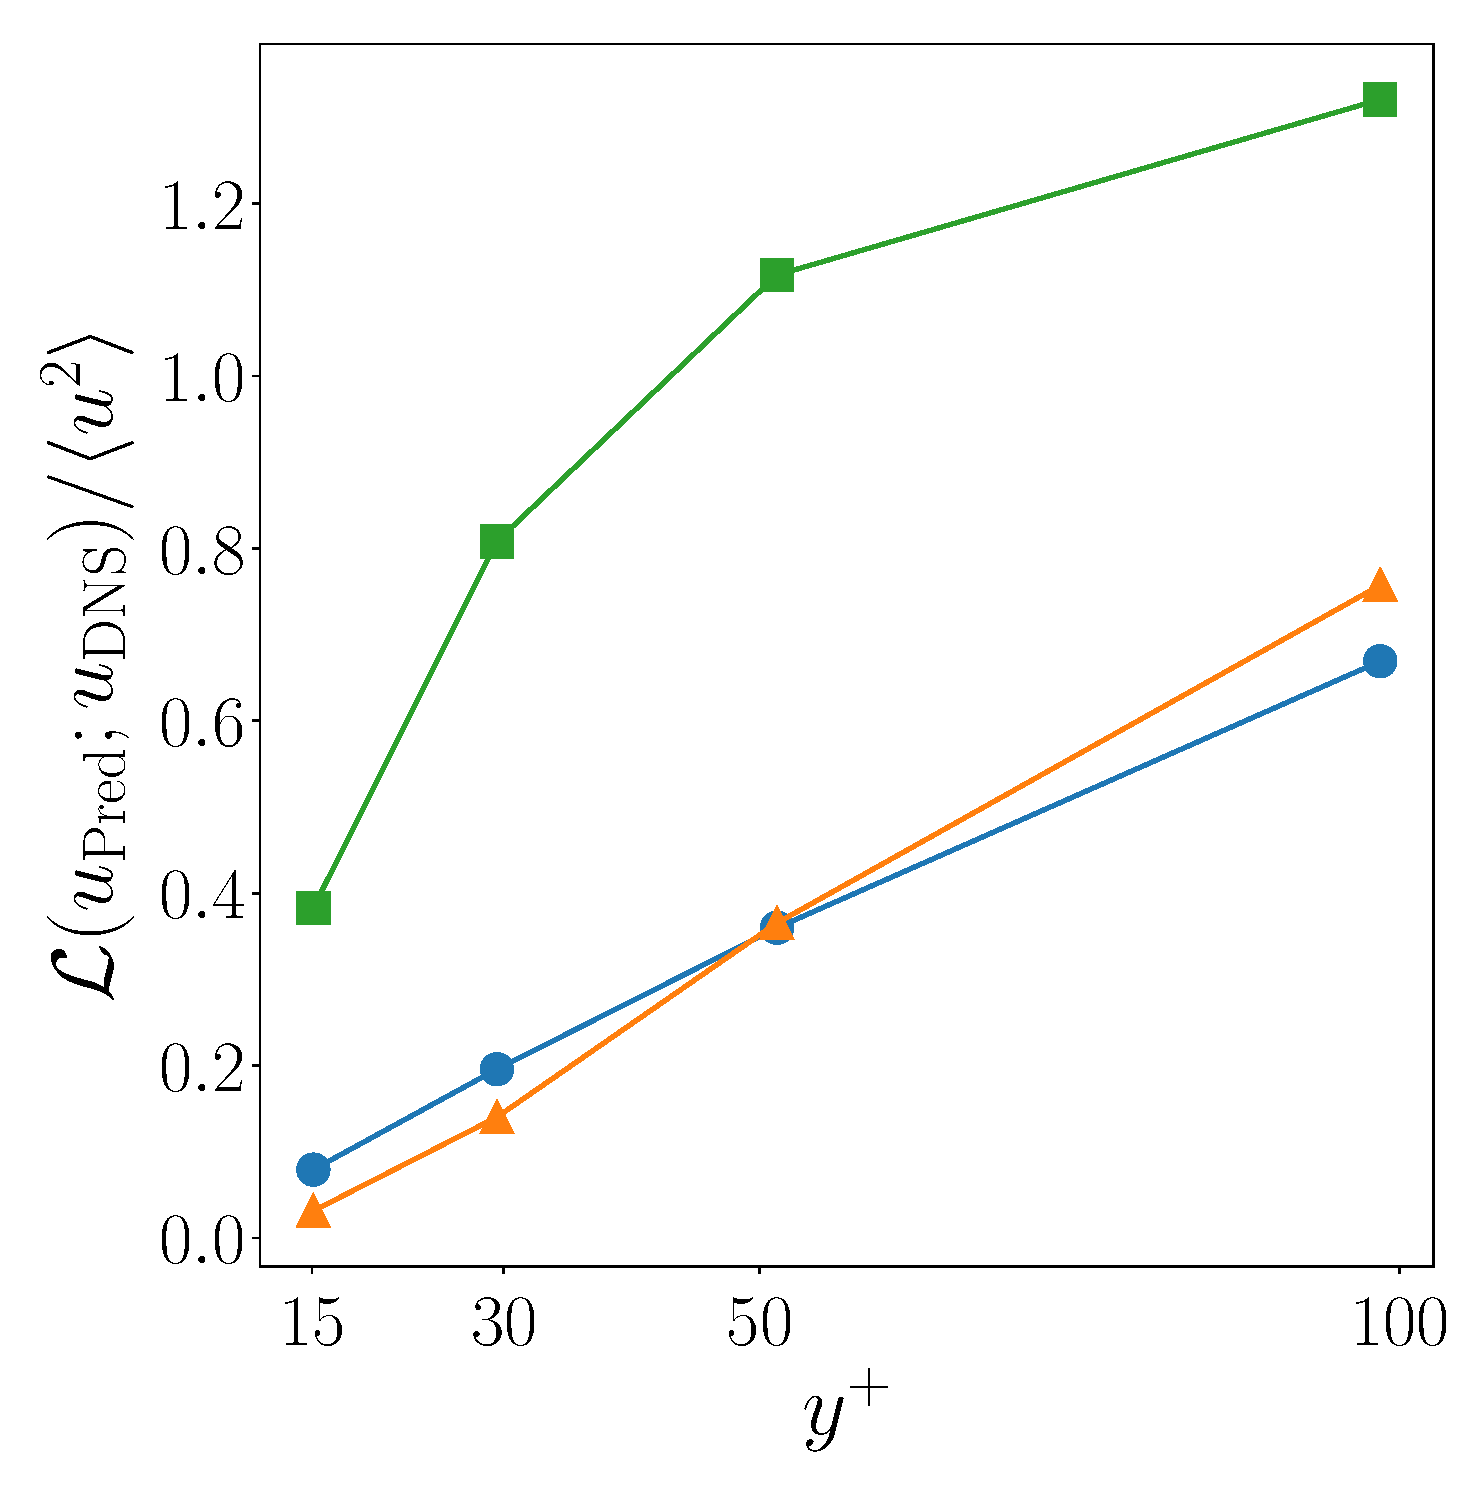
\includegraphics[width=.32\columnwidth]{Ret180/mse_u180_rms_scale.eps}
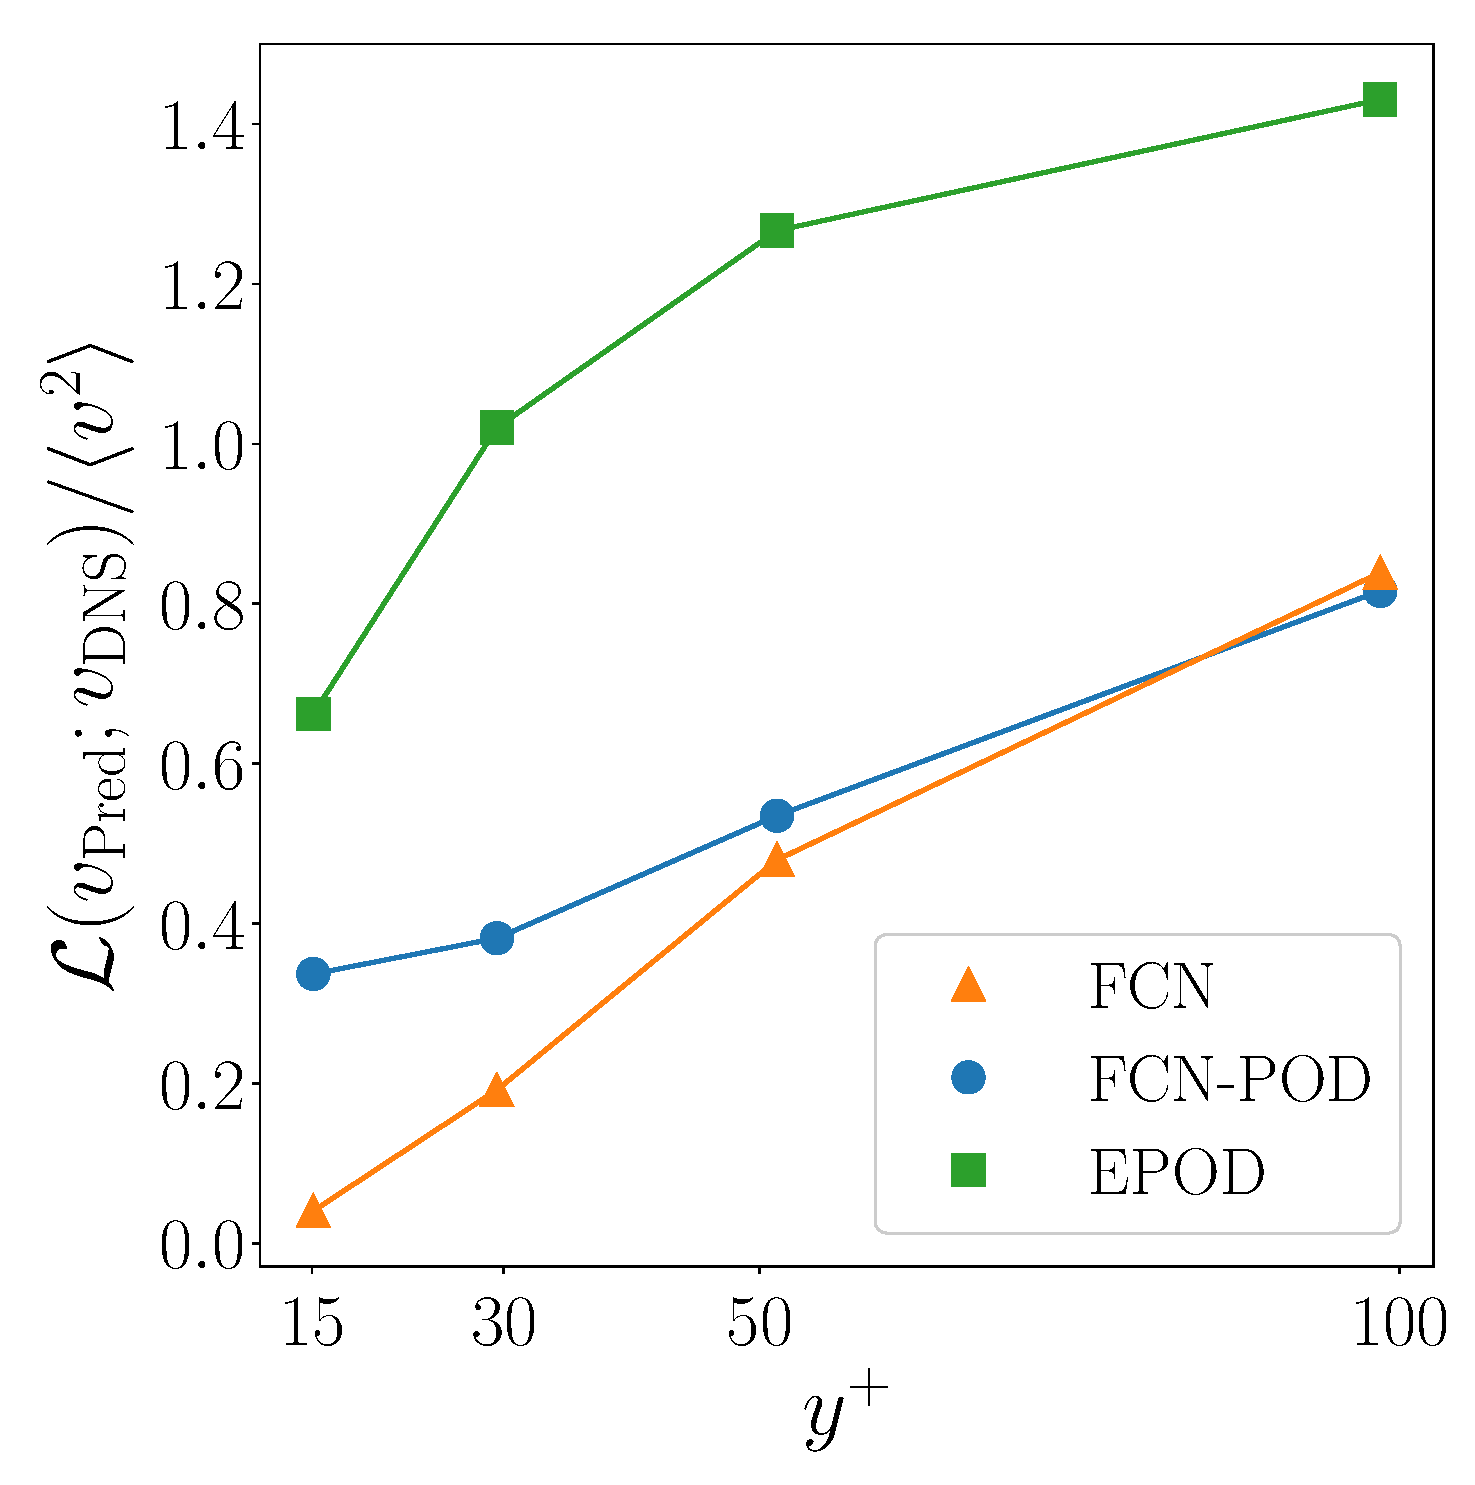
\includegraphics[width=.32\columnwidth]{Ret180/mse_v180_rms_scale.eps}
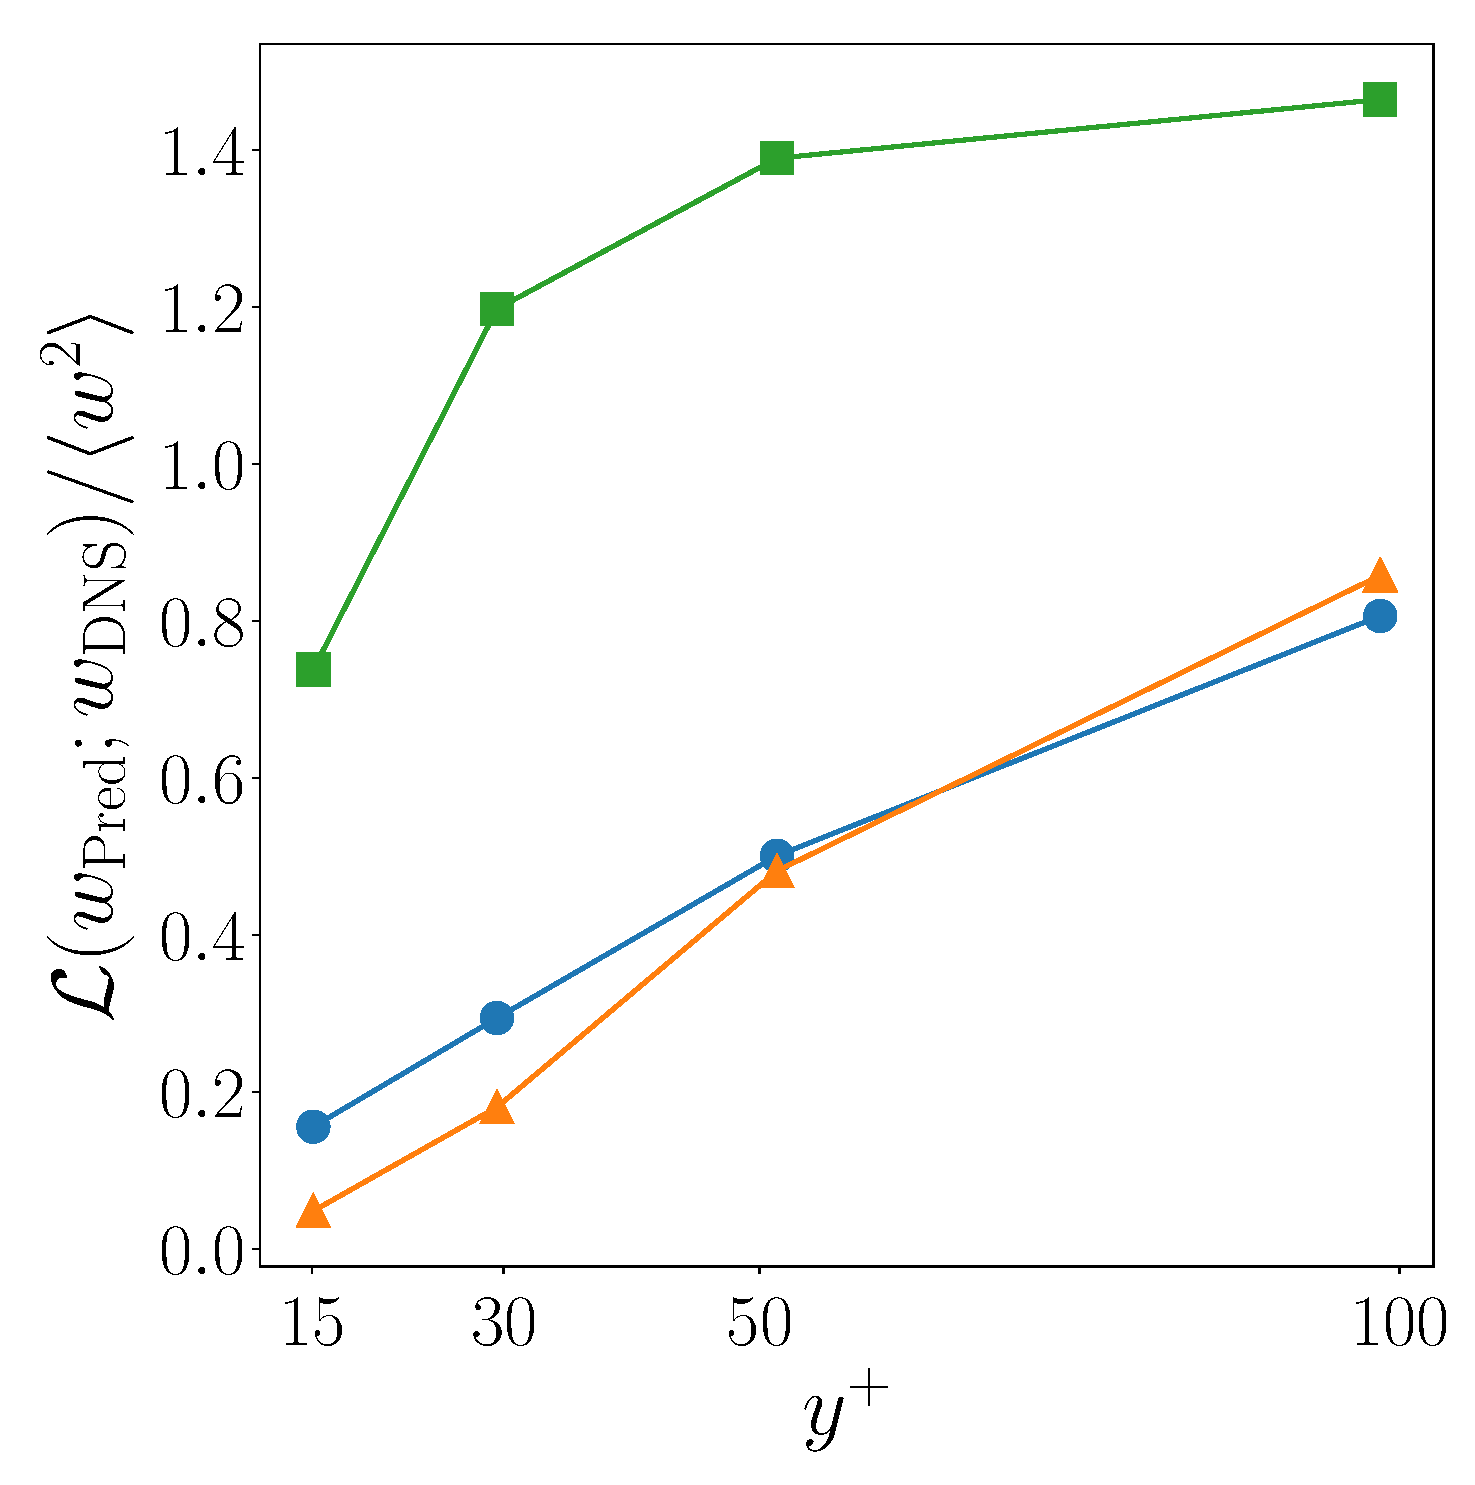
\includegraphics[width=.32\columnwidth]{Ret180/mse_w180_rms_scale.eps}
\end{center}
\caption{\label{fig:loss180} Mean-squared-error in the instantaneous fields (scaled with the corresponding RMS components) predicted by the three models at $Re_{\tau} = 180$, for the streamwise (left), wall-normal (middle) and spanwise (right) velocity fluctuations.}
\end{figure}

% Multiple component predictions
The FCN architecture reported by \citet{guastoni2020prediction} would only predict the streamwise velocity component of the velocity field at the target $y^+$.
The addition of the two other components implies that the FCN has multiple outputs that need to be optimized at the same time. We note that adding the two additional fluctuating components as outputs leads to slightly less accurate predictions with respect to those reported by \citet{guastoni2020prediction} for one single output.
This is not surprising, since the capacity of the network remained unchanged, however we tested a variation of the model architecture based on this observation, in order to have more layers dedicated to the prediction of each individual component.
This network variation has a common part, identical to the original FCN up to the 4$^{\text{th}}$ convolutional layer, in which the weights are optimized using the information from the error gradients computed for all the outputs.
The last two convolution operations are replicated for each velocity component and the weights of these layers are updated only with the error associated to the respective output.
Such a network, despite its higher capacity, provided worse predictions.
A strong causal relation between the different components of the velocity~\citep{lozano2020causality} can be a possible explanation for this result, which shows that updating all the weights with information from the three components at the same time can be beneficial for the quality of the predictions.
Note that it is not trivial to design an architecture able to provide the best trade-off between single-component predictions and usage of the information from all the components, and obtaining such an architecture would require further investigation.
For the FCN-POD model the multiple-component predictions were obtained as discussed by \citet{guemes2019sensing}.
The temporal POD coefficients can be projected on spatial POD modes involving the three velocity components, thus requiring only one output to predict the three fluctuations.
The network architecture is different than the one used by \citet{guemes2019sensing}, since it predicts directly all the needed time coefficients for each snapshot.
While the final fully-connected layer included in the network architecture by \citet{guemes2019sensing} improves the robustness of the prediction, the FCN-POD implementation used here has a much smaller number of weights, thus significantly reducing the computational cost, and retains a larger number of POD modes (and thus more energy).


\begin{figure}
\begin{center}
\includegraphics[width=\textwidth]{Ret550/u_550smaller_fields.png}
\end{center}
\caption{\label{fig:field_comp550} Comparison of the streamwise fluctuation fields at $Re_{\tau} = 550$, scaled with the corresponding $u_\mathrm{RMS}$, from EPOD (1$^{\text{st}}$ row), FCN-POD (2$^{\text{nd}}$ row), reference DNS (3$^{\text{rd}}$ row) and FCN (4$^{\text{th}}$ row). Results at $y^+=15$ (1$^{\text{st}}$ column), $y^+=30$ (2$^{\text{nd}}$ column), $y^+=50$ (3$^{\text{rd}}$ column) and $y^+=100$ (4$^{\text{th}}$ column).}%\highlight{AG: This instantaneous fields seem too positive (too red). LG: the mean of the field is not zero, but slightly positive, moreover the overall distribution of u in the dataset is skewed, it has positive mode.}% \highlight{LG: currently in draft mode otherwise it takes forever to load}}
\end{figure}

Predictions of the streamwise fluctuation fields from the various methods at $Re_{\tau} = 550$ are shown in figure~\ref{fig:field_comp550}, while the results for the wall-normal and spanwise components are presented in Appendix~\ref{appA}.
Despite the higher friction Reynolds number, the FCN maintains a performance similar to the one achieved for $Re_{\tau}=180$, at all wall-normal locations.
Note that the FCN has the same architecture as the lower-Reynolds-number case, {\it i.e.} it has the same number of trainable parameters, while in the case of the FCN-POD approach, the network was modified to reconstruct approximately the same amount of energy as at $Re_{\tau}=180$.
Despite the higher number of employed subdomains, the tiling is more apparent at $Re_{\tau}=550$.
The prediction performance of the FCN-POD model degrades less quickly than the FCN when moving away from the wall, however the latter still performs better at $y^+=50$, as shown in figure~\ref{fig:loss550}.
On the other hand, the EPOD also exhibits similar error levels as those reported for $Re_{\tau}=180$, except at $y^+=15$, where the reconstruction of the streamwise-fluctuation field is significantly worse.

\begin{figure}
\begin{center}
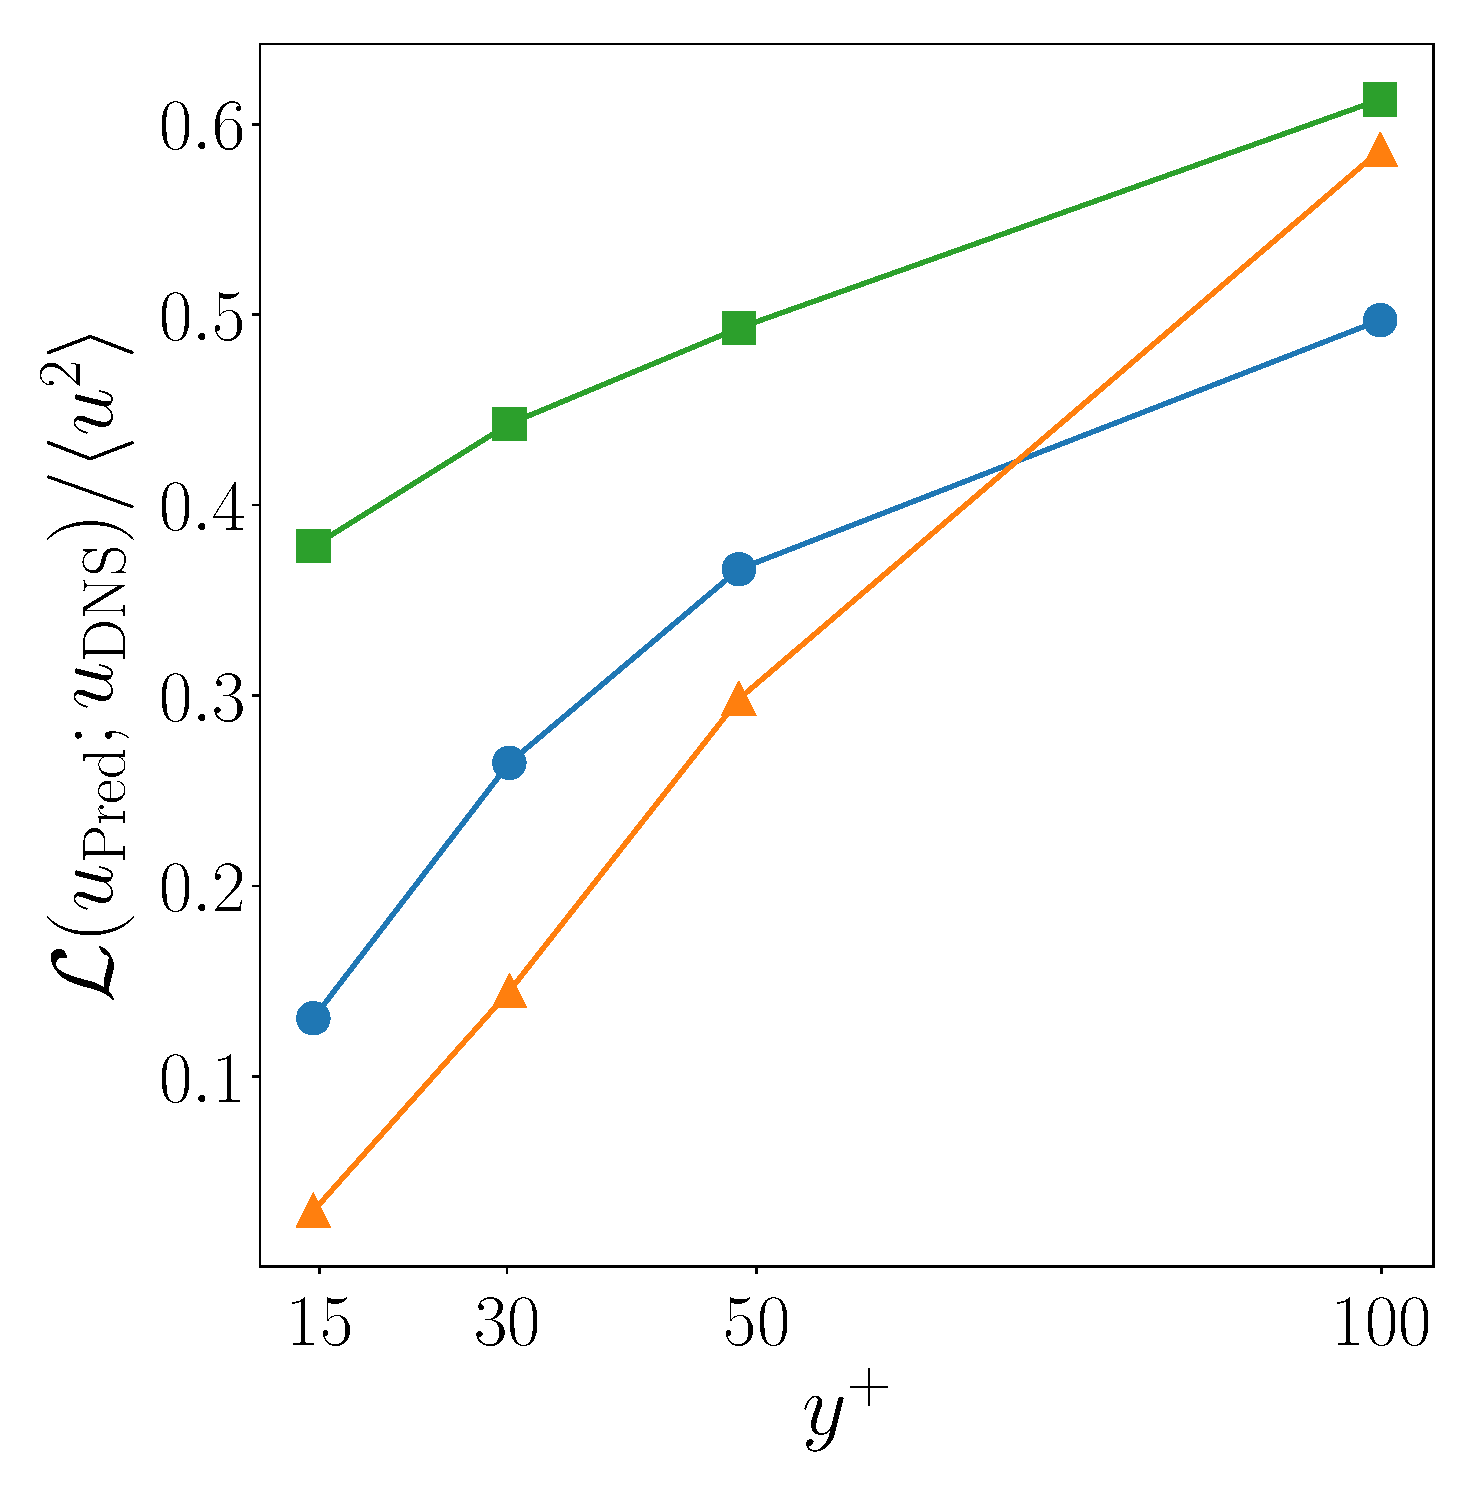
\includegraphics[width=.32\columnwidth]{Ret550/mse_u550_rms_scale.eps}
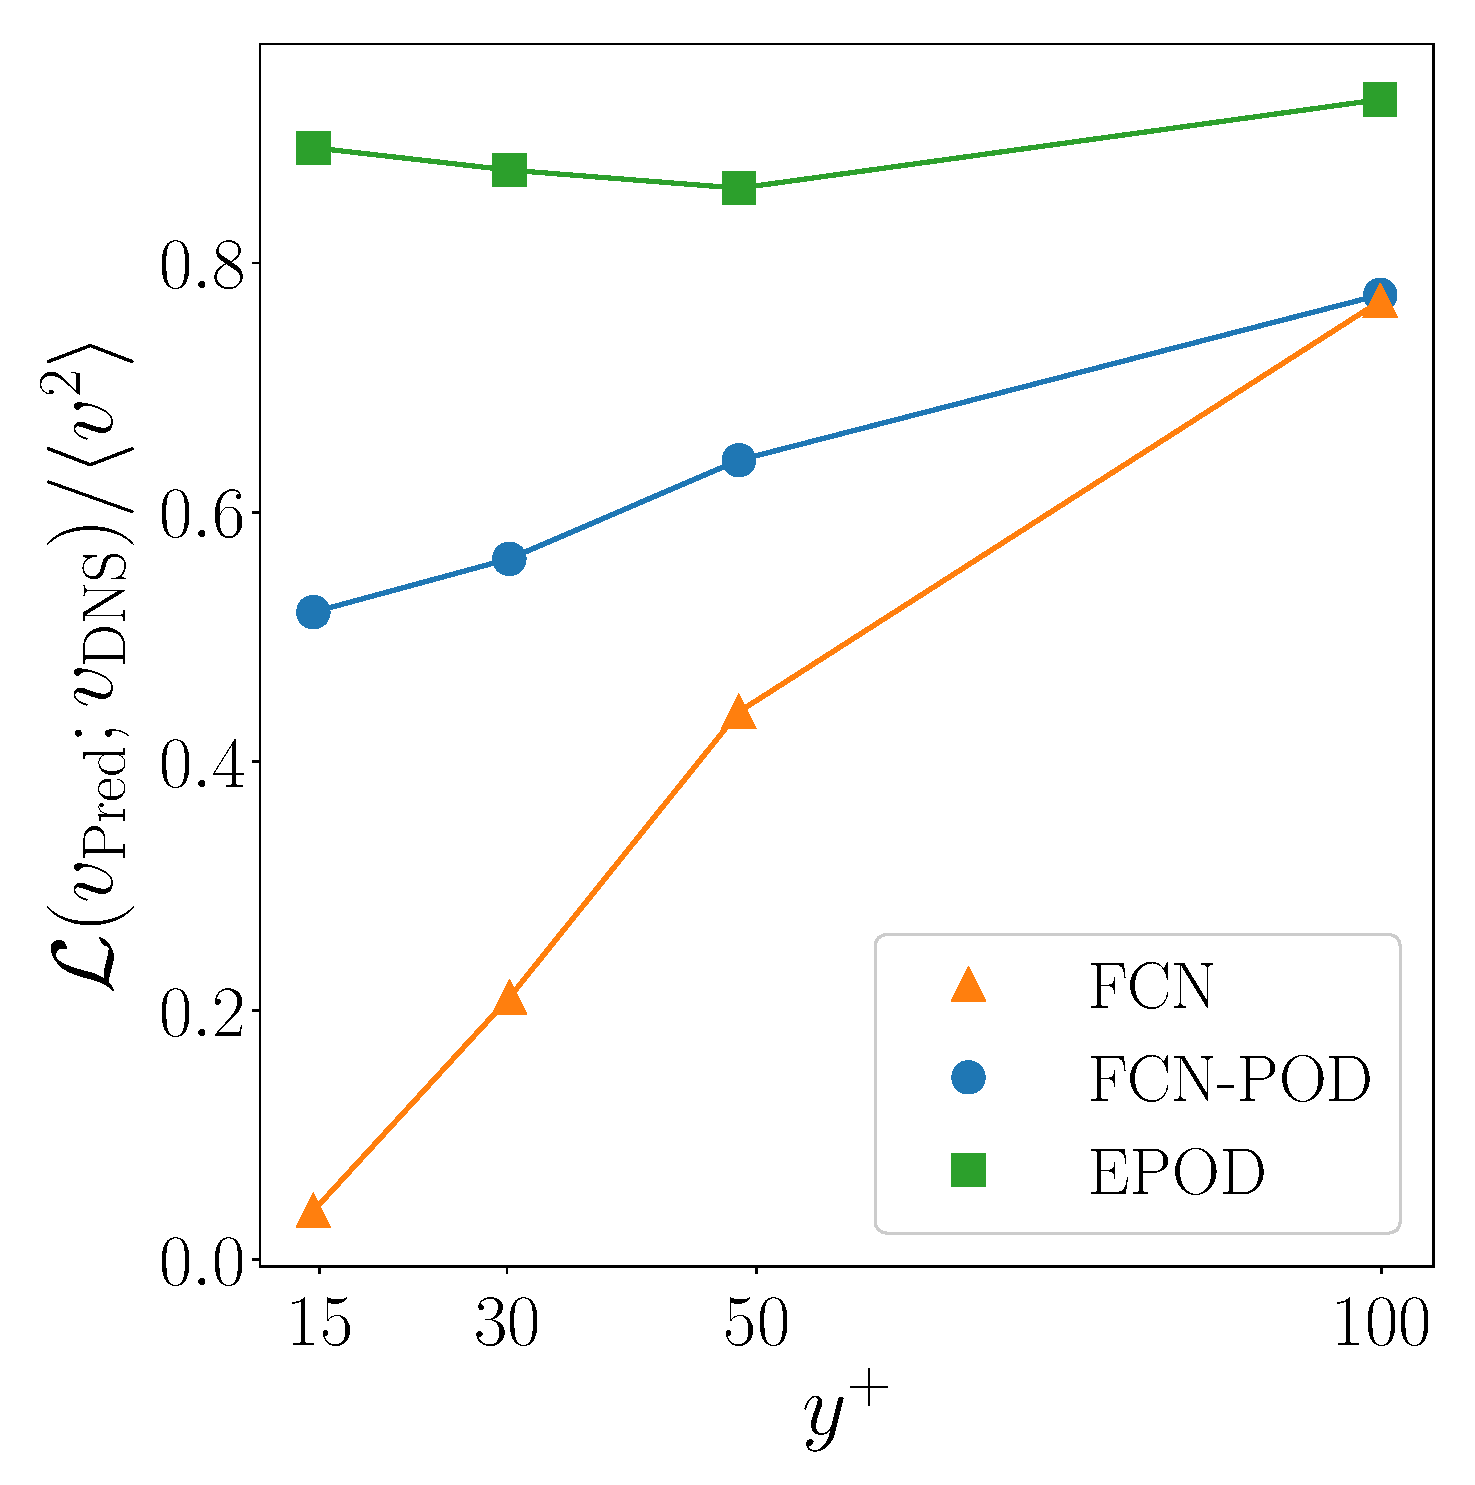
\includegraphics[width=.32\columnwidth]{Ret550/mse_v550_rms_scale.eps}
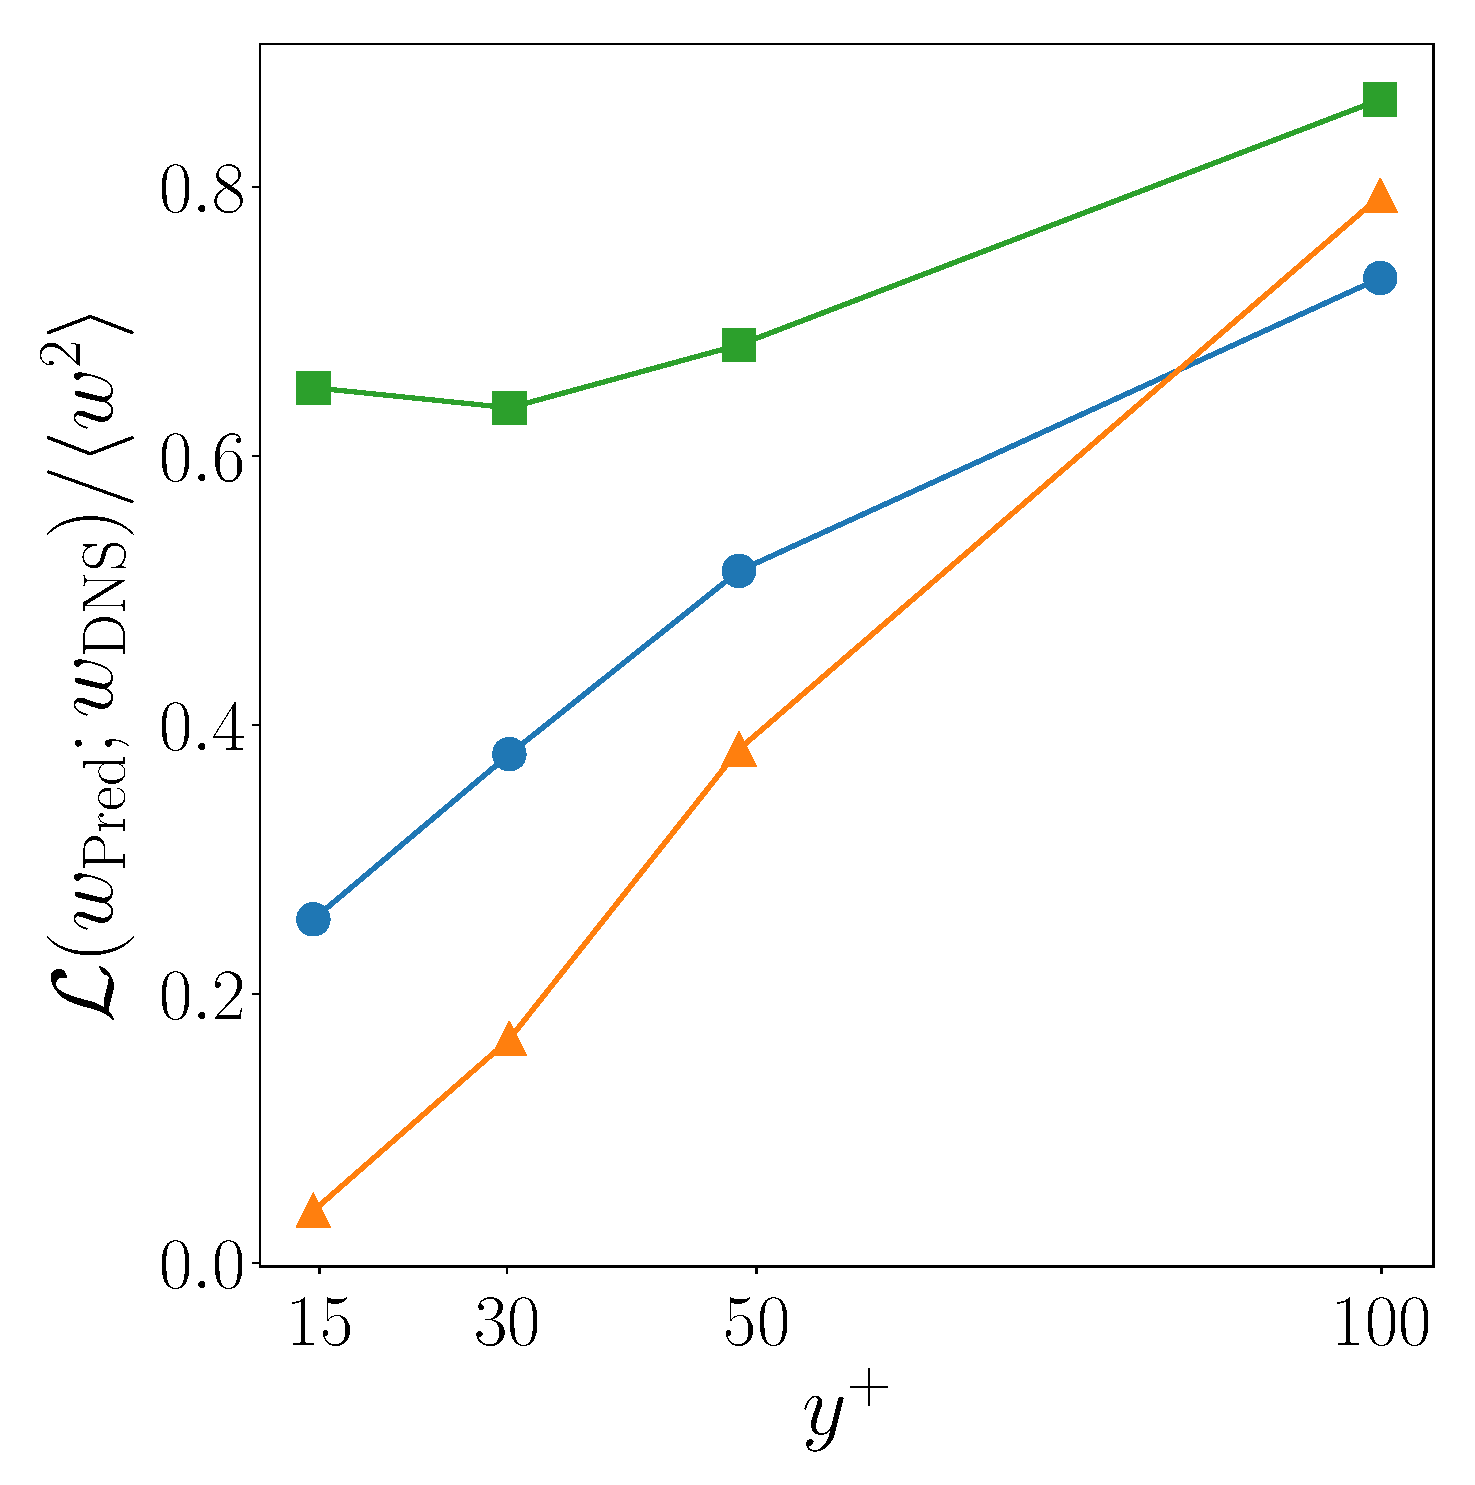
\includegraphics[width=.32\columnwidth]{Ret550/mse_w550_rms_scale.eps}
\end{center}
\caption{\label{fig:loss550} Mean-squared-error in the instantaneous fields (scaled with the corresponding RMS components) predicted by the three models at $Re_{\tau}=550$, for the streamwise (left), wall-normal (middle) and spanwise (right) velocity fluctuations.}
\end{figure}


\subsubsection{Inclination of coherent structures} \label{sss:shift}
The coherent structures in wall-bounded turbulence are inclined~\citep{marusic2007reynolds}, with a slope that can be computed by finding the maximum spatial correlation $\mathcal{R}_{ij}(\delta x)$ between the inputs at the wall (index $i$) and the outputs (index $j$), with $\delta x$ representing the distance in the streamwise direction at which the correlation is computed.
By including a streamwise \textit{shift} in the output fields, it is possible to obtain the maximum correlation at $\delta x=0$, ensuring that the footprint of the coherent structure is included in the receptive field of the output.
The use of such a shift was also discussed by \citet{sasaki2019transfer} in a similar context.
By considering the maximum correlation between the wall-shear stress in the streamwise direction and the streamwise velocity at a certain $y^+$, we obtain an angle:
\begin{equation}
 \theta_{\mathrm{shift}} = \tan^{-1}\left(\frac{\arg\,\max_{\delta x} R_{11}(\delta x)}{\delta y}\right) \approx 11^{\circ}
\end{equation}
\noindent at $Re_{\tau}=180$, where $\delta y$ indicates the considered distance from the wall.
 The obtained value is slightly lower than previous observations~\citep{marusic2007reynolds,sasaki2019transfer}, possibly because of the low Reynolds number.
 The inclusion of the shift information has been tested using two alternative implementations: first, by modifying the target output field, {\it i.e.} considering a field that has been sampled later in the simulation, although the accuracy of the introduced shift is limited by the value of the sampling period.
 The second approach makes use of the periodicity of the output fields, which are translated in the streamwise direction until the maximum correlation is obtained at $\delta x=0$.
 This approach allows to more accurately introduce the shift, however in this case the underlying hypothesis is that the shift is sufficiently small so that temporal dynamics modify the flow in a negligible manner.
 None of the two shift implementations provided the expected improvement, and we observed a significant degradation of the prediction performance.
 These results could possibly be explained by the fact that coherent structures of different size have different inclinations, and imposing a single value is detrimental for the overall network performance, despite having chosen the angle that provides the maximum spatial correlation.
 Furthermore, the quality of the predictions is measured using the MSE between the prediction and the reference: this error indicator considers all wavelengths at the same time, without considering how the different wavelengths are affected by the shift.
 Further investigation of this aspect, also at higher $Re_{\tau}$, will be conducted in future work.

\subsection{Predictions of turbulence statistics}\label{ss:stat}

By averaging over the fields obtained from the neural-network models and EPOD, it is possible to evaluate the turbulence statistics of the predicted flow.
First we consider the dataset at $Re_{\tau}=180$: the predicted RMS fluctuations of the three components are shown in figure~\ref{fig:stats180}, together with the reference DNS profiles.
The error in these statistical quantities is defined as:
%
\begin{equation}
    E_\mathrm{RMS}^+(u) = \frac{\left| u_\mathrm{RMS,Pred}^+ - u_\mathrm{RMS,DNS}^+ \right|}{u_\mathrm{RMS,DNS}^+},
\end{equation}
for the streamwise component, and similarly for the other two components.
As above, the subscripts `DNS' and `Pred' refer to the reference and predicted profiles, respectively.
An important premise is that neither of the neural-network-based models is explicitly optimized to reproduce the statistics of the original simulation.
This prevents the neural networks from learning only the average behaviour of the flow, however the predictions may be less statistically accurate, with the aim of maximizing the instantaneous performance.
Note that here we favor instantaneous performance because our motivation is to use non-intrusive sensing for closed-loop flow control.

The prediction errors in the various RMS profiles are summarized in table~\ref{tab:RMS_err_180}, and they are averaged over the different training runs for the FCN and FCN-POD models.
Note that the average is performed over the fluctuation-intensity values and not on the predictions, because that would alter the statistical properties of the predicted flow fields.
The comparison of the errors from the different models shows that the statistical performance mimics the one observed for the instantaneous predictions at $y^+=15$ and $y^+=30$, with the FCN performing better than the FCN-POD and EPOD models.
Furthermore, the FCN model provides a similar performance for the fluctuations of all three velocity components, while POD-based methods are more accurate in the predictions of $u_\mathrm{RMS}^+$.
This is related to the choice of not scaling the different velocity components in the FCN-POD and EPOD approaches, and the fact that near the wall the most energetic dynamics of the flow are in the streamwise direction.
Taking into account the standard deviation in the results of the neural-network-based methods, the three models provide similar error levels at $y^+=50$. At $y^+=100$ the scenario is opposite to what we observed close to the wall: the FCN exhibits the highest errors, while the EPOD provides the best results.
The error in the prediction of $u_\mathrm{RMS}^+$ from the FCN-POD model is between those of the two other models, while the wall-normal and spanwise intensities are closer to the errors from the FCN, due the reasons outlined above.

\begin{figure}
\begin{center}
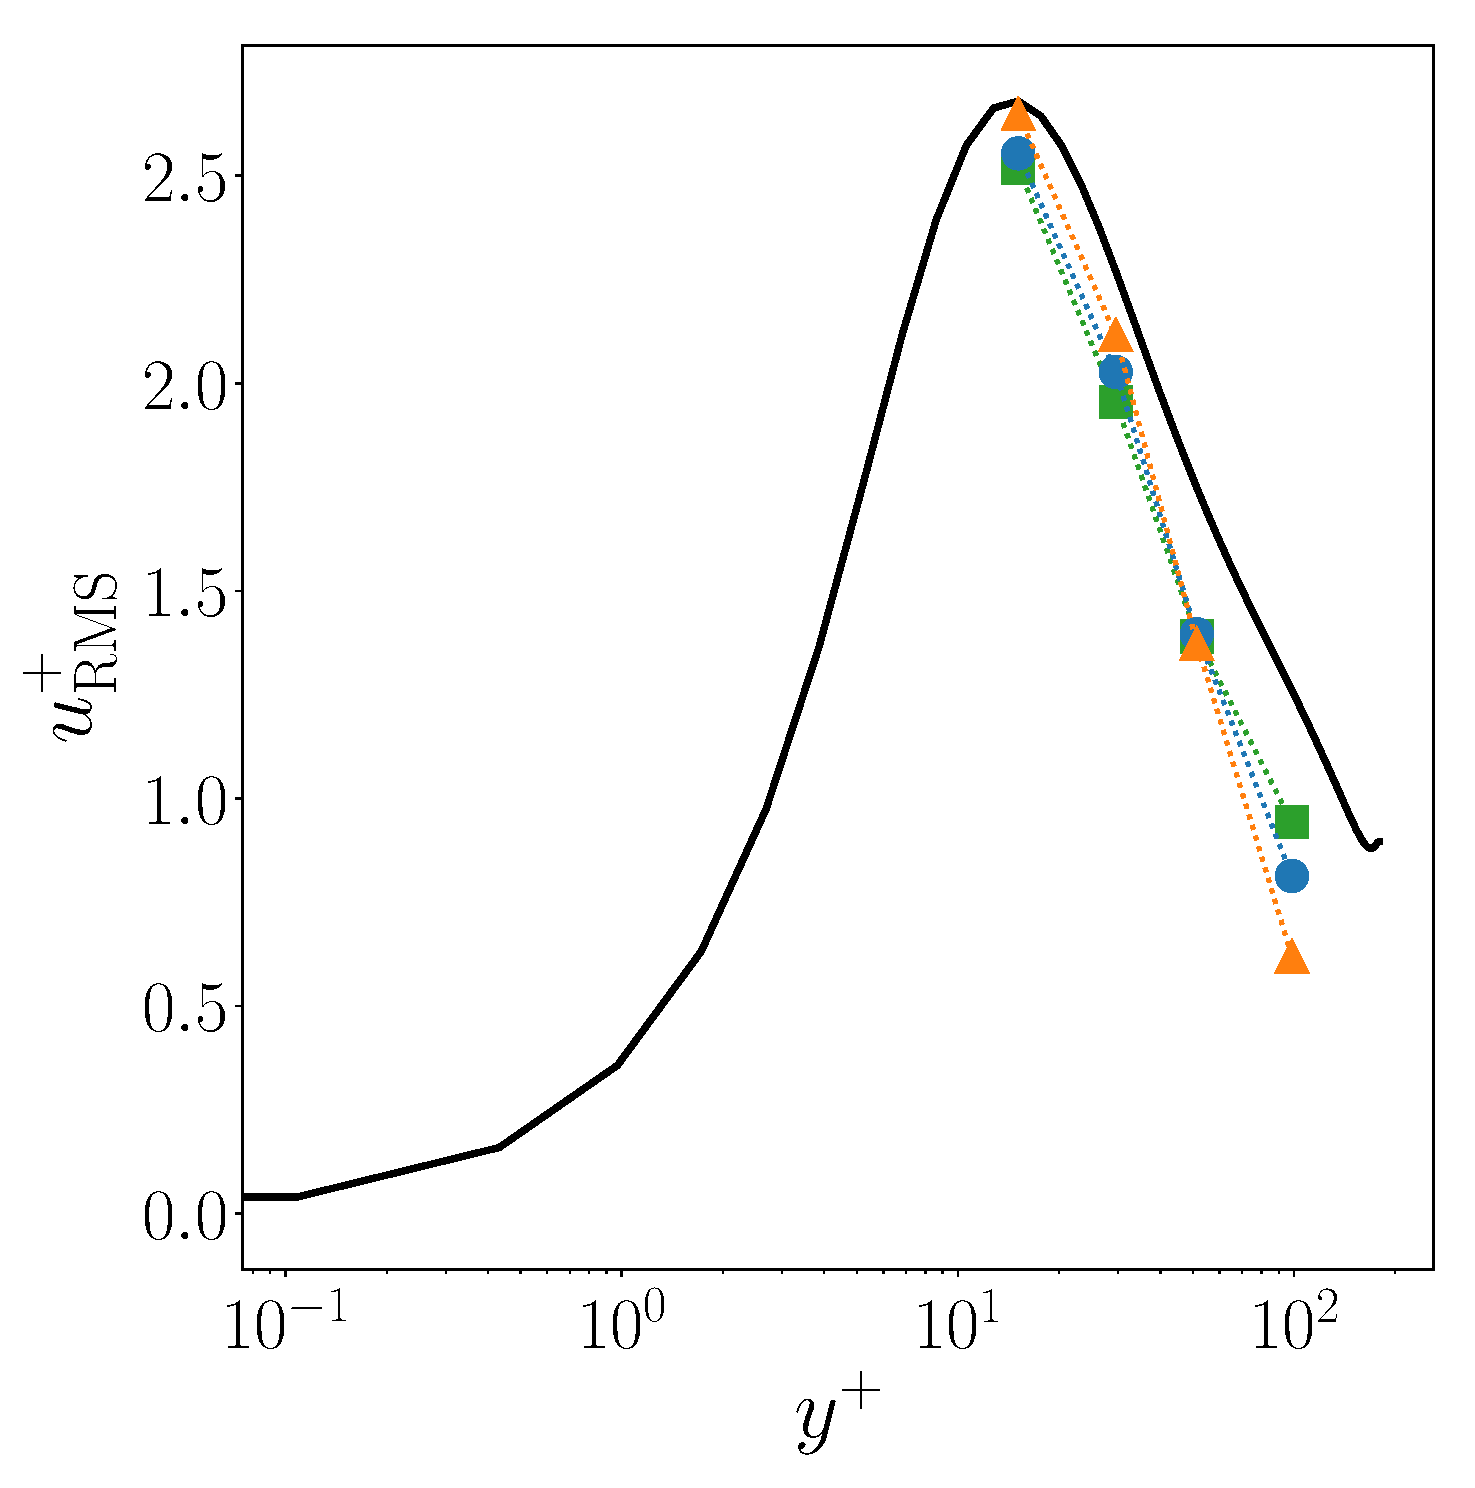
\includegraphics[width=.32\columnwidth]{Ret180/uu180.eps}
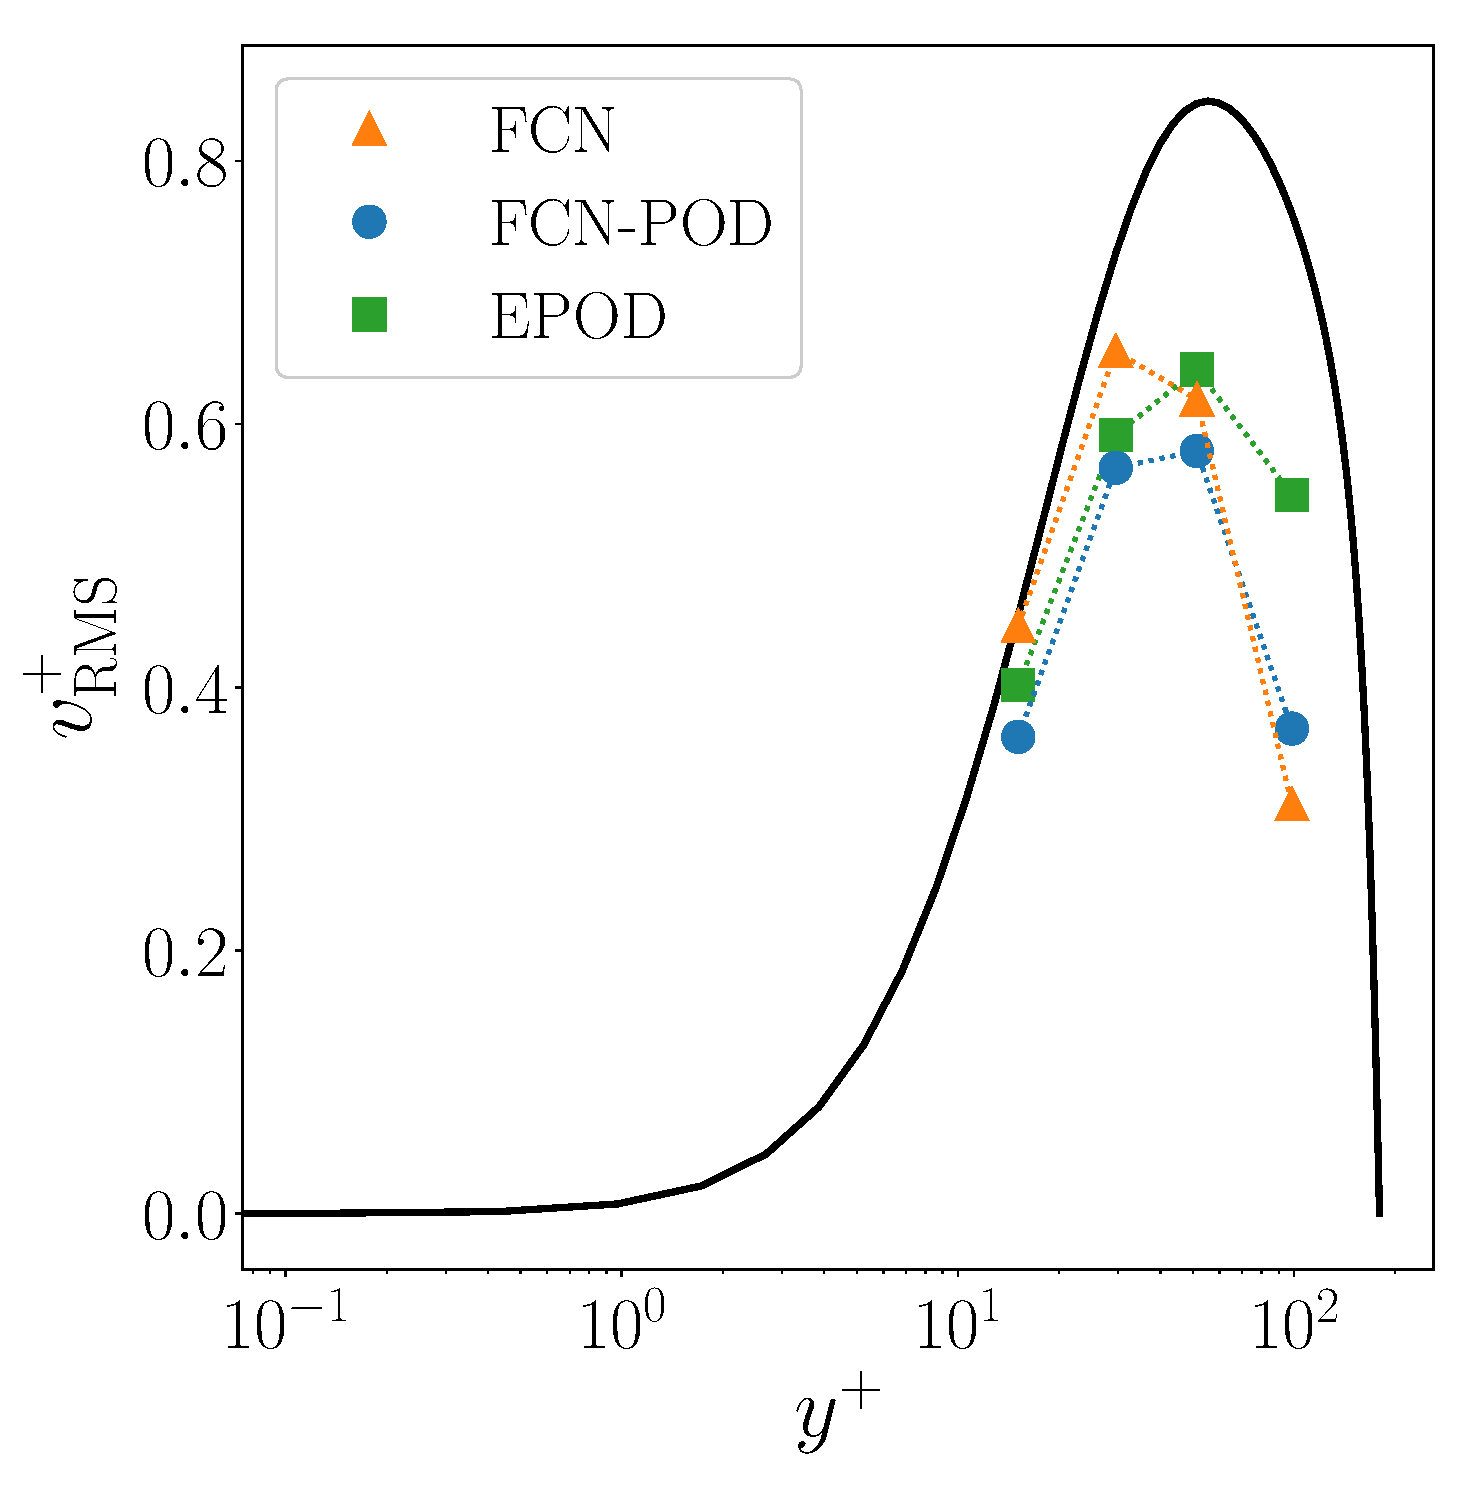
\includegraphics[width=.32\columnwidth]{Ret180/vv180.eps}
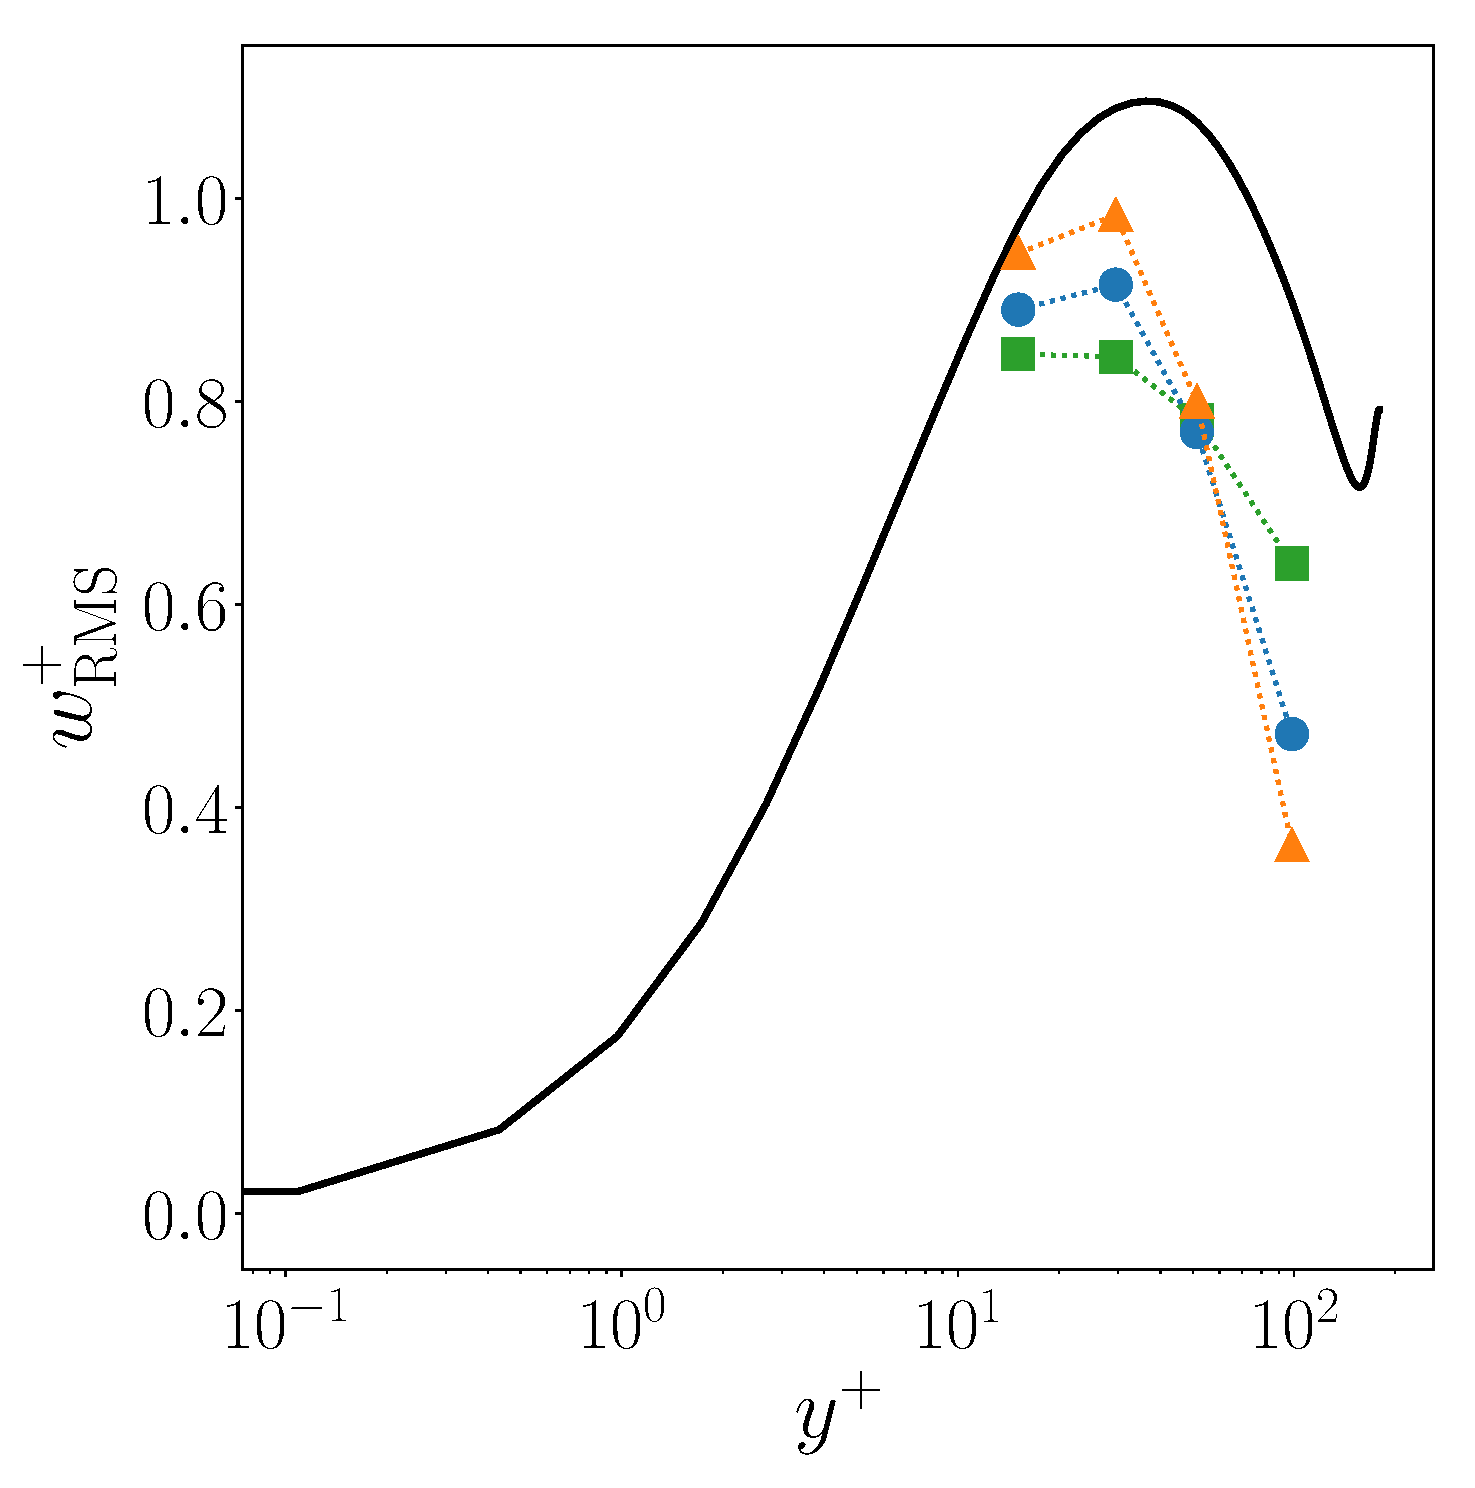
\includegraphics[width=.32\columnwidth]{Ret180/ww180.eps}
\end{center}
\caption{\label{fig:stats180} Comparison between the DNS (\full) and the predictions of streamwise (left),
 wall-normal (middle) and spanwise (right) velocity
fluctuations at $Re_{\tau} = 180$.}
\end{figure}

\begin{table}
\centering
\resizebox{\columnwidth}{!}{%
    \begin{tabular}{l l*{4}{c}}
        $E_\mathrm{RMS}^+(\cdot)\ [\%]$ &         & $y^+=15$                       & $y^+=30$                     & $y^+=50$           & $y^+=100$          \\[0.3cm]

                                        & EPOD    & $\phantom{0}6.03~~~~~~~~~~~$   & $13.87~~~~~~~~~~~$           & $20.50~~~~~~~~~~~~$ & $25.15~~~~~~~~~~~~$ \\
        $u$                             & FCN     & $\phantom{0}1.16~(\pm 0.74)$   & $\phantom{0}6.79~(\pm 1.31)$ & $21.47~(\pm 1.97)~$ & $50.82~(\pm 2.19)~$ \\
                                        & FCN-POD & $\phantom{0}4.70~(\pm 0.02)$   & $10.70~(\pm 0.02)$           & $20.15~(\pm 0.03)~$ & $35.46~(\pm 0.02)~$ \\[0.3cm]

                                        & EPOD    & $11.68~~~~~~~~~~~$             & $18.89~~~~~~~~~~~$           & $23.97~~~~~~~~~~~~$ & $28.10~~~~~~~~~~~~$ \\
        $v$                             & FCN     & $\phantom{0}1.74~(\pm 1.00)$   & $10.18~(\pm 1.67)$           & $26.66~(\pm 0.76)~$ & $59.05~(\pm 1.61)~$ \\
                                        & FCN-POD & $20.29~(\pm 0.02)$             & $22.32~(\pm 0.02)$           & $31.32~(\pm 0.01)~$ & $51.48~(\pm 0.04)~$ \\[0.3cm]

                                        & EPOD    & $13.01~~~~~~~~~~~$             & $22.48~~~~~~~~~~~$           & $27.27~~~~~~~~~~~~$  & $28.72~~~~~~~~~~~~$ \\
        $w$                             & FCN     & $\phantom{0}2.79~(\pm 0.36)$   & $\phantom{0}9.65~(\pm 1.07)$ & $25.60~(\pm 1.214)$  & $59.59~(\pm 1.310)$ \\
                                        & FCN-POD & $\phantom{0}8.50~(\pm 0.04)$   & $15.95~(\pm 0.06)$           & $28.38~(\pm 0.004)$  & $47.42~(\pm 0.001)$ \\
    \end{tabular}%
    }
    \caption{Percentage error in the prediction of the various RMS fluctations at the different wall-normal locations. Results at $Re_{\tau} = 180$.}
    \label{tab:RMS_err_180}
\end{table}

The statistical analysis is repeated also for the models trained at $Re_{\tau} = 550$, with the predicted RMS fluctuations shown in figure~\ref{fig:stats550} and the relative error with respect to the reference simulation in table~\ref{tab:RMS_err_550}.
FCN-based models do not show a significant variation in the prediction of the streamwise fluctuations with respect to the results at $Re_{\tau}=180$, whereas the EPOD exhibits higher errors at this Reynolds number (also in the other two fluctuating components).
The FCN has a consistent behaviour also for the fluctuations in the \textit{y}- and \textit{z}-directions, however the FCN-POD performs slightly worse than before, following the same trend but with higher error levels.
The FCN-POD method outperforms the FCN approach only at $y^+=100$, confirming the results of the instantaneous performance at $Re_{\tau} = 550$.

\begin{figure}
\begin{center}
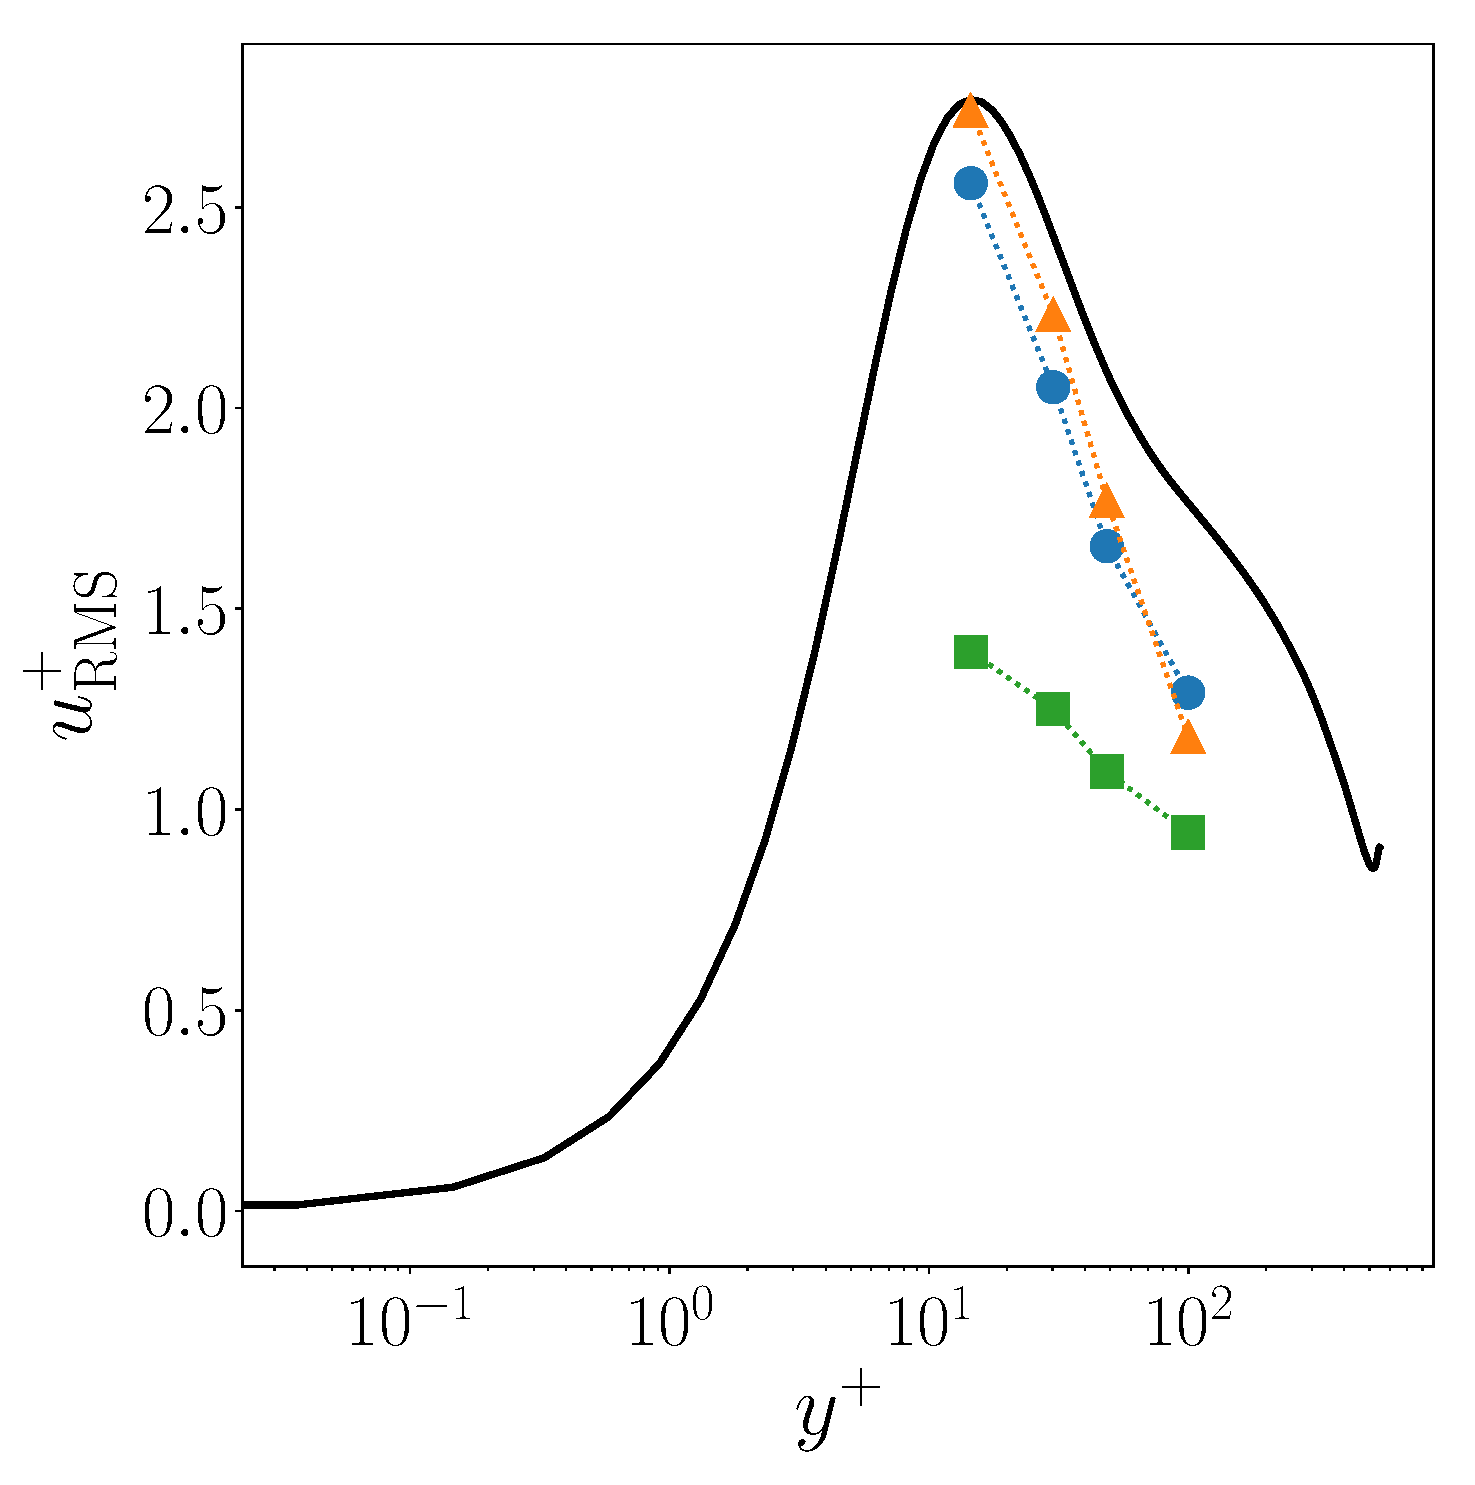
\includegraphics[width=.32\columnwidth]{Ret550/uu550_v3.eps}
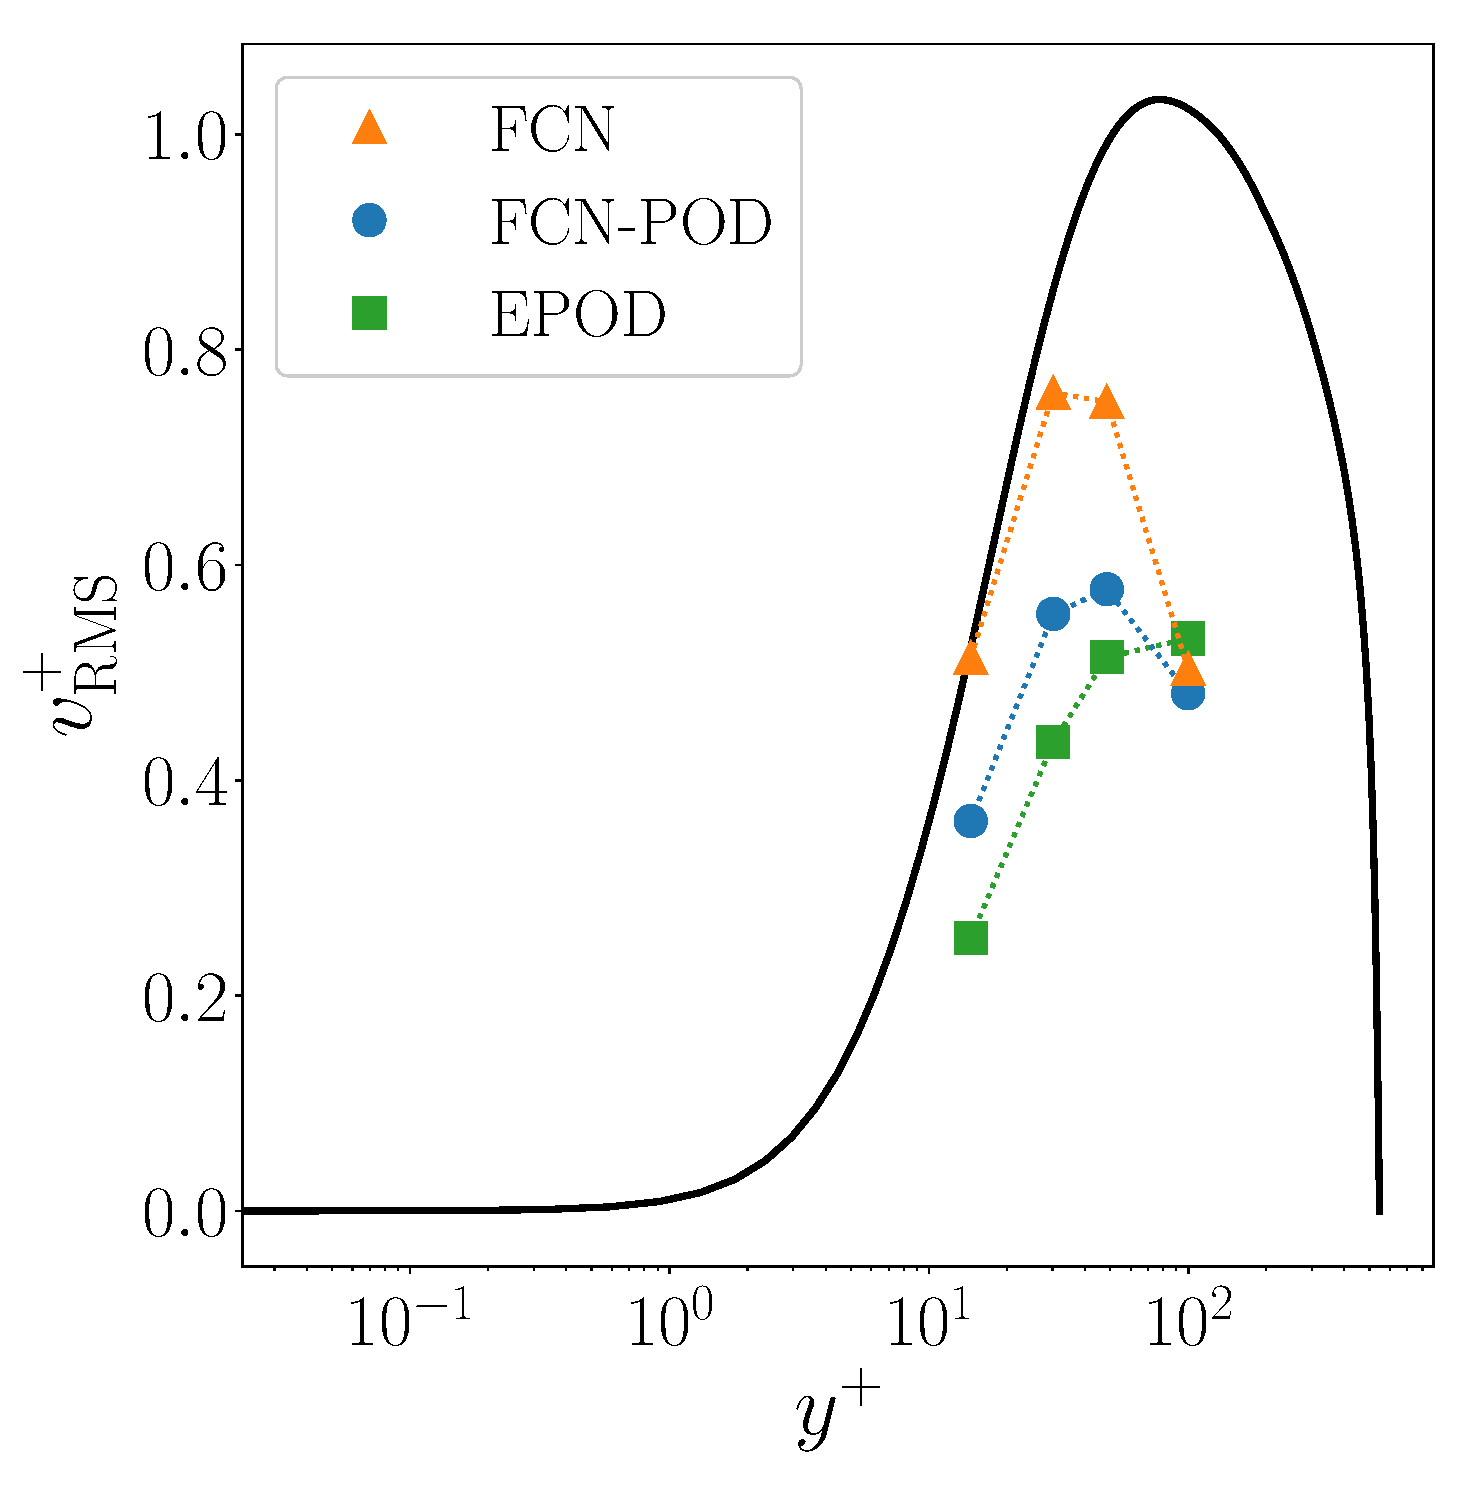
\includegraphics[width=.32\columnwidth]{Ret550/vv550_v3.eps}
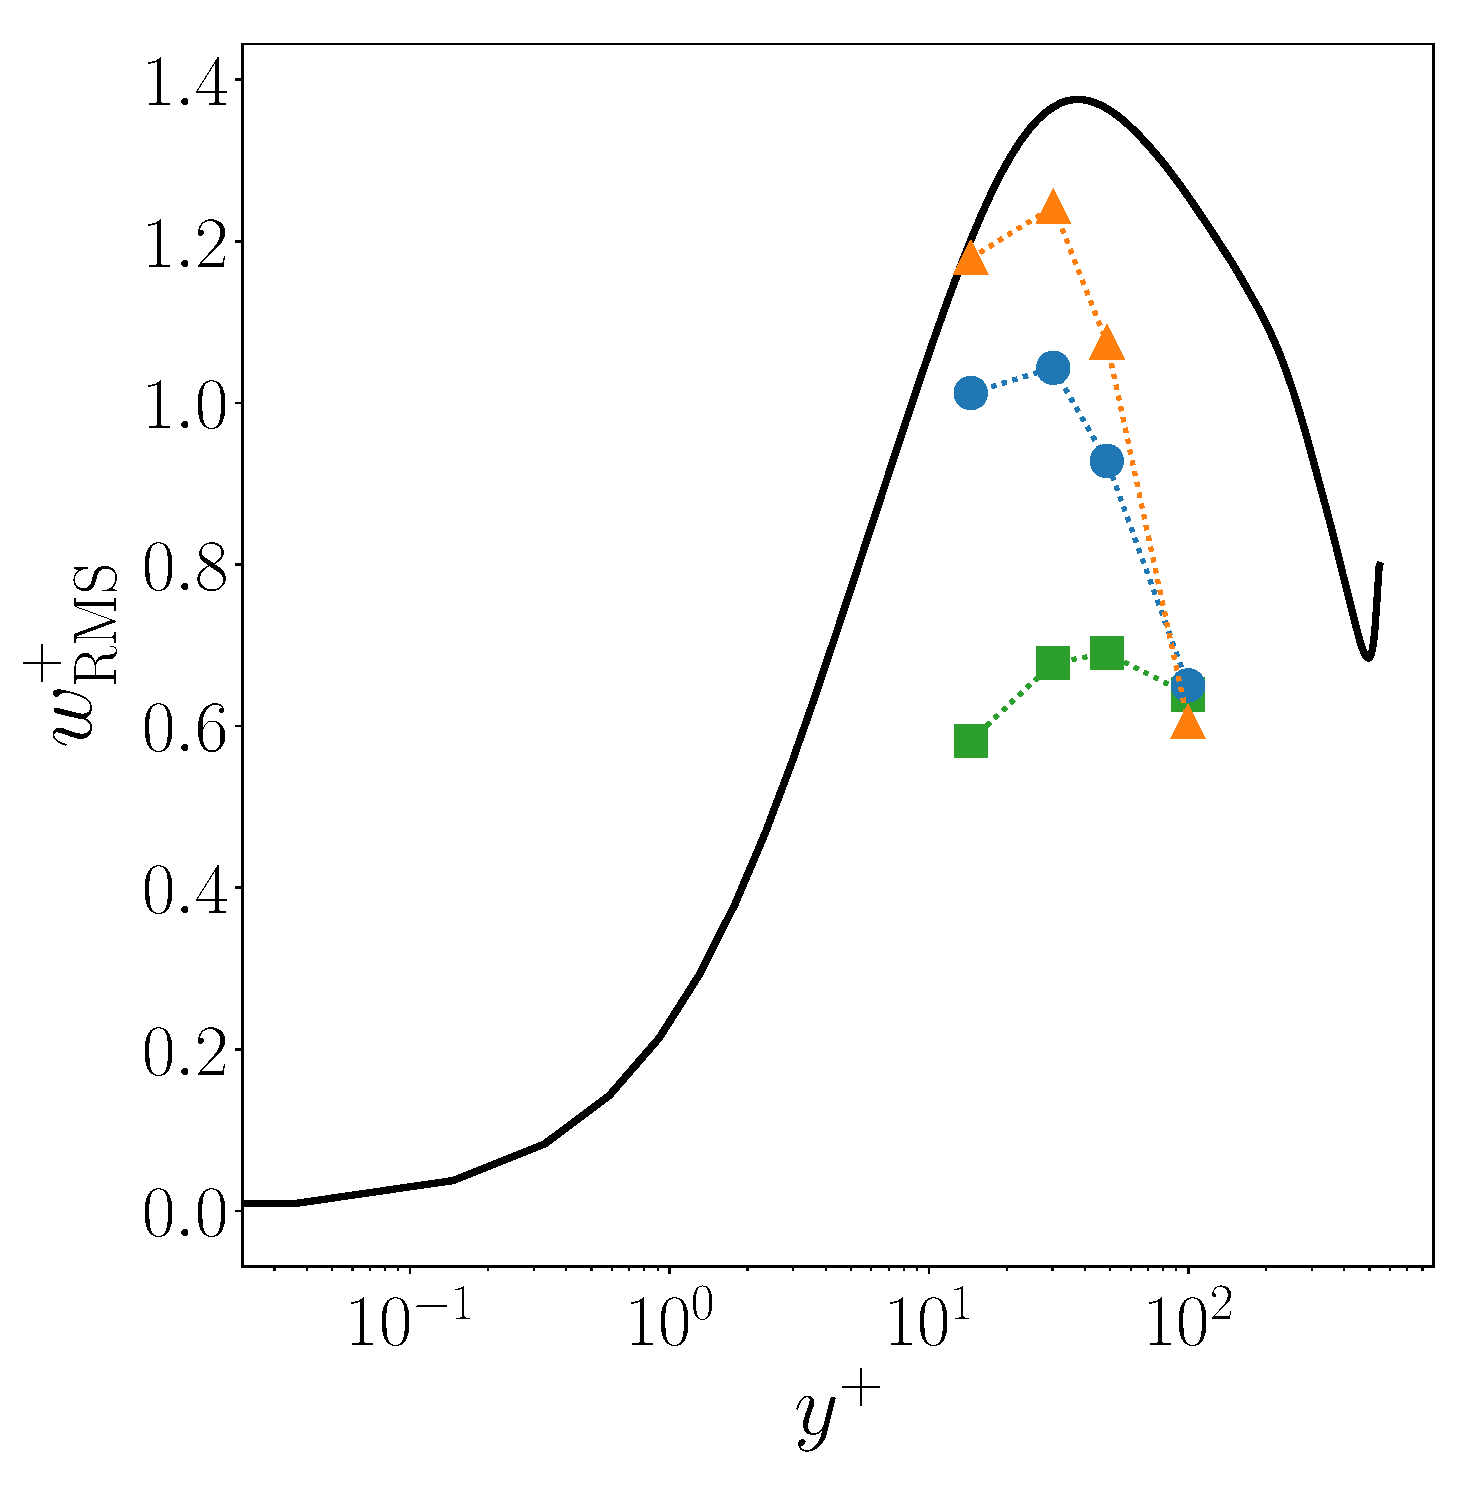
\includegraphics[width=.32\columnwidth]{Ret550/ww550_v3.eps}
\end{center}
\caption{\label{fig:stats550} Comparison between the DNS (\full) and the predictions of streamwise (left),
 wall-normal (middle) and spanwise (right) velocity
fluctuations at $Re_{\tau} = 550$.}
\end{figure}

\begin{table}
\centering
\resizebox{\columnwidth}{!}{%
    \begin{tabular}{l l*{4}{c}}
        $E_\mathrm{RMS}^+(\cdot)\ [\%]$ &         & $y^+=15$                  & $y^+=30$                     & $y^+=50$                      & $y^+=100$          \\[0.3cm]

                                     & EPOD    & $49.69~~~~~~~~~~$            & $48.53~~~~~~~~~~~$           & $47.62~~~~~~~~~~~$            & $46.53~~~~~~~~~~~$ \\
        $u$                          & FCN     & $0.98~(\pm 0.66)$            & $\phantom{0}8.10~(\pm 0.62)$ & $15.33~(\pm 0.22)$            & $33.06~(\pm 0.30)$ \\
                                     & FCN-POD & $7.53~(\pm 0.27)$            & $15.53~(\pm 0.39)$           & $20.75~(\pm 0.85)$            & $26.79~(\pm 0.36)$ \\[0.3cm]

                                     & EPOD    & $51.57~~~~~~~~~~$            & $49.13~~~~~~~~~~~$           & $48.13~~~~~~~~~~~$            & $48.07~~~~~~~~~~~$ \\
        $v$                          & FCN     & $\phantom{0}1.74~(\pm 0.11)$ & $11.21~(\pm 1.41)$           & $24.20~(\pm 1.38)$            & $50.82~(\pm 0.26)$ \\
                                     & FCN-POD & $30.73~(\pm 0.06)$           & $35.20~(\pm 0.09)$           & $41.75~(\pm 0.10)$            & $53.04~(\pm 0.18)$ \\[0.3cm]

                                     & EPOD    & $51.56~~~~~~~~~~$            & $50.35~~~~~~~~~~~$           & $49.42~~~~~~~~~~~$            & $49.08~~~~~~~~~~~$ \\
        $w$                          & FCN     & $\phantom{0}1.86~(\pm 0.60)$ & $\phantom{0}9.03~(\pm 0.31)$ & $21.21~(\pm 1.27)$            & $51.83~(\pm 0.38)$ \\
                                     & FCN-POD & $15.74~(\pm 0.05)$           & $23.63~(\pm 0.07)$           & $31.97~(\pm 0.10)$            & $48.20~(\pm 0.24)$ \\
    \end{tabular}%
    }
    \caption{Percentage error in the prediction of the various RMS fluctations at the different wall-normal locations. Results at $Re_{\tau}=550$.}
    \label{tab:RMS_err_550}
\end{table}

\subsection{Predictions of power-spectral density}\label{ss:spec}
\begin{figure}
    \centerline{\includegraphics[width=384pt]{Ret180/spectra_re180large.pdf}}
    \caption{Pre-multiplied two-dimensional power-spectral densities for $Re_{\tau}=180$. The contour levels contain 10\%, 50\% and 90\% of the maximum DNS power-spectral density. Shaded contours refer to the reference data, while contour lines refer to \lcap{.-}{fcn} FCN, \lcap{--}{FCN-POD} FCN-POD and \lcap{:}{epod} EPOD predictions, respectively.}
    \label{fig:spectra180}
\end{figure}

The energetic scales present in the predicted fields, as well as their associated energy, are compared with those in the reference DNS data through spectral analysis.
In figure~\ref{fig:spectra180} we show the pre-multiplied two-dimensional power-spectral density of the streamwise, wall-normal and spanwise fluctuations (denoted by $\phi_{uu}$, $\phi_{vv}$ and $\phi_{ww}$ respectively) at $Re_{\tau}=180$, where $\lambda_{x}$ and $\lambda_{z}$ denote the streamwise and spanwise wavelengths, whereas $k_{x}$ and $k_{z}$ are the corresponding wavenumbers.
These results confirm the observations made in $\S$\ref{ss:inst}: at $y^+=15$, all the considered models are able to correctly predict the energy content of the flow at all wavelengths, with the FCN slightly outperforming the two POD-based approaches.
Note that the FCN-POD model is able to reconstruct the energy content of the flow at wavelengths that are longer than the size of the subdomains, proving that this is not a limiting factor for the model.
However, a small jump, probably due to a lack of smoothness at the edges of the subdomains, can be observed in the streamwise wavelength for the 10\%-energy level in the wall-normal and spanwise components.
These jumps are found at a wavelength $\lambda_x^+ \approx 180$, corresponding to the subdomain size.
At $y^+=30$ there is a slight energy attenuation which becomes increasingly more noticeable when the predicted flow is farther away from the wall.
At $y^+=100$ the POD-based methods perform better than the FCN model, a fact that can be explained by considering two concurring aspects: the first is that POD methods only predict the temporal dynamics of the system, thus the overall energy-scale distribution stored in the POD spatial modes does not need to be predicted.
This allows to reconstruct more than $50\%$ of the flow fields, at least in the streamwise component.
The second aspect is the fact that the receptive field from the FCN method, while sufficient for planes closer to the wall, is not large enough to reproduce the large scales present at larger $y^{+}$.

Figure~\ref{fig:spectra550} reports the reference and predicted power-spectral densities at $Re_{\tau}=550$.
As opposed to what was observed for the instantaneous predictions and the turbulence statistics, the spectra highlight the differences and similarities between the models used for the two Reynolds numbers.
As noted above, the FCN architecture is the same for both $Re_{\tau}$, however this implies that the receptive field is smaller at higher Reynolds number when it is measured in outer units.
This can potentially help in the prediction of the small scales, but it can also be detrimental for the larger scales.
Note that the different size of the receptive field does not seem to affect the predicted energy content of the FCN, which shows the same trends as for the low-$Re_{\tau}$ case.
On the other hand, the spectra of the FCN-POD with $12\times12$ subdomains (the same amount as in the low-$Re_{\tau}$ case, not shown) exhibits spurious periodic peaks due to the tiling.
This observation motivated the increased number of subdomains considered at $Re_{\tau}=550$.
As in the low-$Re_{\tau}$ case, the FCN-POD approach is able to reconstruct the scales larger than the subdomain size, but the countour line exhibits a small jump in the streamwise wavelength for the 10\%-energy level.
This jump appears at a wavelength $\lambda_x^+ \approx 200$, corresponding to the subdomain size employed in the high-$Re_{\tau}$ case.
This jump is also appreciated in the streamwise component at $y^+=15$.
The POD-based approaches are outperformed by the FCN in the range of $y^+=15-50$.
Farther from the wall, the accuracy of the FCN is matched by the FCN-POD method. It is interesting to note that the EPOD does not follow the same attenuation process as the FCN-based methods in the wall-normal and spanwise components.
As one moves farther from the wall, the FCN-based methods fail to reproduce a wider range of small scales, whereas the EPOD exhibits more difficulties predicting the large scales.
When it comes to the spectral peaks far from the wall, while the FCN-based methods produce noisier predictions than in the low-$Re_{\tau}$ case, the EPOD is not able to reproduce that part of the spectra.

\begin{figure}
    \centerline{\includegraphics[width=384pt]{Ret550/spectra_re550large.pdf}}
    \caption{Pre-multiplied two-dimensional power-spectral densities for $Re_{\tau}=550$. The contour levels contain 10\%, 50\% and 90\% of the maximum DNS power-spectral density. Shaded contours refer to the reference data, while contour lines refer to \lcap{.-}{fcn} FCN, \lcap{--}{FCN-POD} FCN-POD and \lcap{:}{epod} EPOD predictions, respectively.}
    \label{fig:spectra550}
\end{figure}

\section{Transfer learning}\label{ss:tl}

A number of more advanced techniques have also started to be adopted from the specialized machine-learning literature and applied to fluid-dynamics research.
One notable example is \textit{transfer learning}~\citep{pan2009survey}, a method that allows to transfer knowledge from one neural-network model to another one, thus reducing the amount data and time required for training.
\citet{guastoni2020prediction} showed that the training time at a given wall-normal location may be significantly reduced if the network parameters are initialized using the optimized parameters of a previously-trained network at another wall-normal location.
Similarly, \citet{kim2020prediction} used the convolutional network trained at a low Reynolds number to predict the flow at a higher Reynolds number.

Transfer learning represents an appealing solution for the main drawback of neural networks, which is the need to train them with a sufficient amount of data.
Training typically requires specialized hardware and in our specific application the computational cost of generating the training and test datasets is not negligible.
Furthermore, this cost grows as $Re_{\tau}$ increases, making the generation of training data through DNS unfeasible at the Reynolds numbers that are relevant for engineering applications.
In this regard, it is important to make an efficient use of the data and the trained models at our disposal.
In this work, the possibility of transferring knowledge between models trained at different friction Reynolds numbers is investigated.
At a fixed wall-normal distance, the weights of the FCN model trained on the dataset at $Re_{\tau} = 180$ are loaded before training the network with the higher-$Re_{\tau}$ dataset.
This is possible because the network has the same amount of trainable parameters in both cases, as noted above.
The learning rate is the only parameter that needs to be modified: a lower value has to be set, in order to prevent the optimizer from diverging too quickly from the weight configuration used for initialization.
While in \citet{guastoni2020prediction} we froze the first layers of the initialized network because the input was the same at the different wall-normal locations, in this case all the layers are trainable because the input distribution changes from one $Re_{\tau}$ to the other one.

The transfer-learning numerical experiments that follow are designed with two objectives in mind.
First, we investigate the effect of using the parameters of previously-trained model to initialize a model that will be trained at a different target $Re_{\tau}$ than the first model.
Second, we verify whether the non-random initialization that we described can potentially improve the training process, reducing the amount of data at higher $Re_{\tau}$ that is needed to achieve the same performance of a model trained from scratch, using the entire training/validation dataset, as we did in section~\ref{ss:results}.
To this end, we initialized a FCN model with the parameters learnt on the $Re_{\tau}=180$ dataset and we trained such model on the full training/validation datasets at $Re_{\tau}=550$.
Subsequently, the same initialization is used for models that are trained on a reduced dataset at $Re_{\tau}=550$, namely 25\% and 50\% of the full dataset.
Differently from the previous sections, only one training run was performed for each case.
In order to compare models trained with datasets of different sizes, we considered the number of weight updates through the optimization algorithm during training.
In figure~\ref{fig:transfer} the validation and test losses are compared for the models trained with the full dataset and a random initialization.
When the initialized model is trained on the full dataset, the performance is consistently better than that of the random initialization, both in terms of validation and test loss.
The improvement is more evident close to the wall, whereas at $y^+=100$ the two models provide approximately the same results after the first 150,000 updates.
Transferring knowledge between different Reynolds numbers is then not only feasible, but also advantageous in terms of performance when the same amount of data is considered.
Note that we kept the same ratio (4:1) when dividing training and validation sets even when the size of the dataset was reduced.
In particular, when 50\% or 25\% of the samples are used, the validation set becomes too small to provide a reliable estimate of the error.
On the other hand, the size of the test dataset is the same as the previous experiments.
Up to $y^+=50$, the initialized networks are able to provide a performance that is very similar to that of the reference model with the same number of updates, with significant savings in terms of amount of data needed to train the network.
On the other hand, at $y^+=100$ a sufficient number of samples becomes a necessary condition to ensure the convergence to an optimal configuration: the loss of the network trained with 50\% of the training dataset does not improve after the first 100,000 updates, while with 25\% of the original dataset the network exhibits overfitting.
The initialized models are able to provide a comparable accuracy also from the statistical point of view, as reported in table~\ref{tab:RMS_err_transfer}.
We stress once again that the networks are not explicitly optimized to reduce the error in the statistics and that small variations in these error figures can be ascribed to the stochastic nature of the optimization algorithm.
Overall, these results demonstrate the feasibility of knowledge transfer from models at different $Re_{\tau}$: with careful tuning of the hyperparameters it should be possible to substantially reduce the training time, as well as the amount of data needed for training.
Although not tested, the transfer between different wall-normal locations described in~\citet{guastoni2020prediction} is still applicable in this case, thus enabling a more efficient prediction of the flow at different wall-normal locations.
\begin{figure}
    \centerline{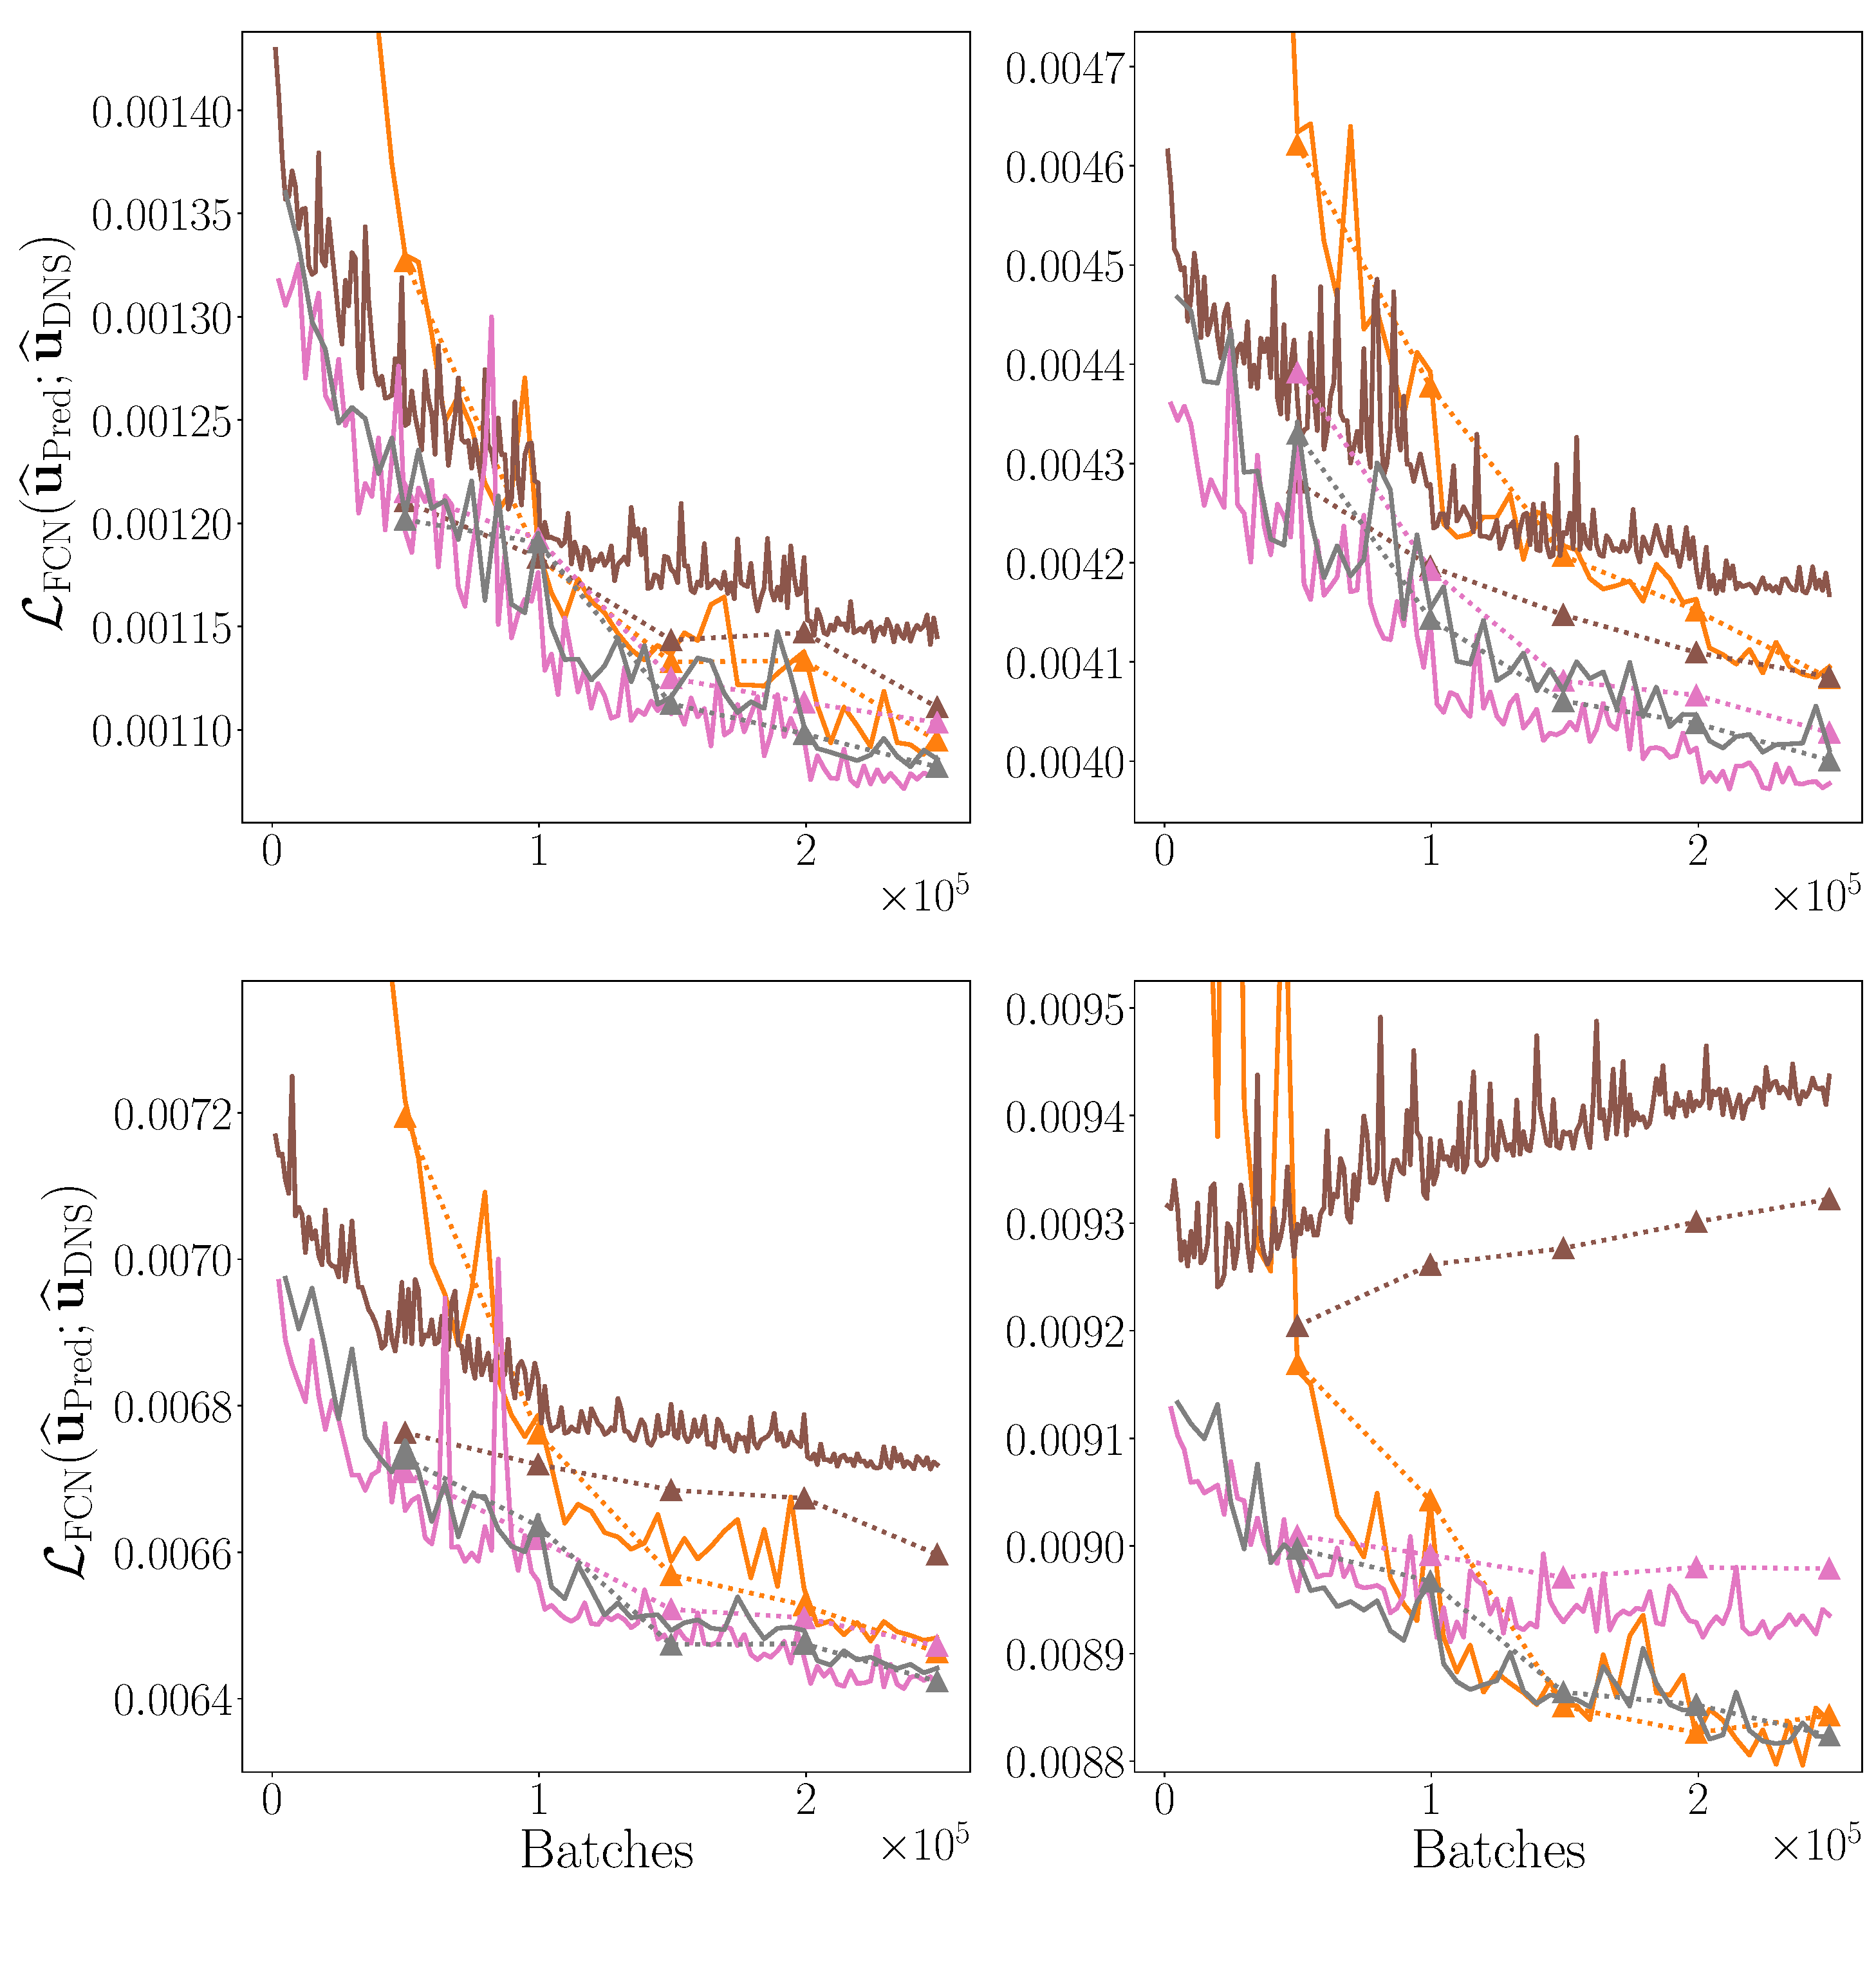
\includegraphics[width=\textwidth]{transfer_learning_v4.eps}}
    \caption{Validation (\full) and test (\dashed) loss in the FCN prediction at (from left to right, top to bottom): $y^+=15$, 30, 50 and 100. Orange represents the models trained with the full dataset and random initialization, grey the models trained with the full dataset and initialized with previously-trained networks, pink and brown represent models initialized with the parameters from the $Re_{\tau}=180$ network, trained with 50\% and 25\% of the original dataset, respectively.}
    \label{fig:transfer}
\end{figure}

\begin{table}
\centering
\resizebox{\columnwidth}{!}{%
    \begin{tabular}{l l*{4}{c}}
        $E_\mathrm{RMS}^+(\cdot)\ [\%]$ &          & $y^+=15$                    & $y^+=30$                     & $y^+=50$                      & $y^+=100$                    \\[0.3cm]

        $u$                             & Ref.     & $0.98~(\pm 0.66)$           & $8.10~(\pm 0.62)$            & $15.33~(\pm 0.22)$            & $33.06~(\pm 0.30)$           \\
                                        & 100\%    & $1.22\phantom{~(\pm 0.00)}$ & $7.15\phantom{~(\pm 0.00)}$  & $16.09\phantom{~(\pm 0.00)}$  & $32.75\phantom{~(\pm 0.00)}$ \\
                                        & 50\%     & $2.94\phantom{~(\pm 0.00)}$ & $7.11\phantom{~(\pm 0.00)}$  & $16.33\phantom{~(\pm 0.00)}$  & $34.11\phantom{~(\pm 0.00)}$ \\
                                        & 25\%     & $1.15\phantom{~(\pm 0.00)}$ & $7.74\phantom{~(\pm 0.00)}$  & $14.78\phantom{~(\pm 0.00)}$  & $33.78\phantom{~(\pm 0.00)}$ \\[0.3cm]

        $v$                             & Ref.     & $1.74~(\pm 0.11)$           & $11.21~(\pm 1.41)$           & $24.20~(\pm 1.38)$            & $50.82~(\pm 0.26)$           \\
                                        & 100\%    & $1.86\phantom{~(\pm 0.00)}$ & $9.40\phantom{0~(\pm 0.00)}$ & $24.40\phantom{~(\pm 0.00)}$  & $51.59\phantom{~(\pm 0.00)}$ \\
                                        & 50\%     & $2.40\phantom{~(\pm 0.00)}$ & $9.46\phantom{0~(\pm 0.00)}$ & $25.96\phantom{~(\pm 0.00)}$  & $50.90\phantom{~(\pm 0.00)}$ \\
                                        & 25\%     & $1.71\phantom{~(\pm 0.00)}$ & $11.33\phantom{~(\pm 0.00)}$ & $23.15\phantom{~(\pm 0.00)}$  & $50.43\phantom{~(\pm 0.00)}$ \\[0.3cm]

        $w$                             & Ref.     & $1.86~(\pm 0.60)$           & $9.03~(\pm 0.31)$            & $21.21~(\pm 1.27)$            & $51.83~(\pm 0.38)$           \\
                                        & 100\%    & $1.75\phantom{~(\pm 0.00)}$ & $8.65\phantom{~(\pm 0.00)}$  & $21.05\phantom{~(\pm 0.00)}$  & $53.04\phantom{~(\pm 0.00)}$ \\
                                        & 50\%     & $2.61\phantom{~(\pm 0.00)}$ & $7.70\phantom{~(\pm 0.00)}$  & $21.34\phantom{~(\pm 0.00)}$  & $52.60\phantom{~(\pm 0.00)}$ \\
                                        & 25\%     & $1.22\phantom{~(\pm 0.00)}$ & $9.67\phantom{~(\pm 0.00)}$  & $20.35\phantom{~(\pm 0.00)}$  & $49.75\phantom{~(\pm 0.00)}$ \\
    \end{tabular}%
    }
    \caption{Percentage error in the prediction of the various RMS fluctations at the different wall-normal locations from models initialized with parameters from the $Re_{\tau}=180$ FCN. The statistics of the different initialized models are computed after 250,000 updates, and they are shown together the models with full dataset and random initialization, which is included as a reference. Results at $Re_{\tau}=550$.}
    \label{tab:RMS_err_transfer}
\end{table}

\section{Conclusions}\label{ss:conclu}

In this work, we introduced and compared two different models based on fully-convolutional neural networks, for prediction of the velocity fluctuations at a given wall-normal distance, using quantities measured at the wall as inputs.
The FCN and FCN-POD models are improved versions of previous architectures, used by \citet{guastoni2020prediction} and \citet{guemes2019sensing}, respectively.
Both of them are able to provide predictions in very good agreement with the reference data, simulated by means of the pseudo-spectral DNS code SIMSON~\citep{chevalier2007pseudo}, up to $y^{+}=50$.
Such an agreement is verified by comparing the error in instantaneous predictions, turbulence statistics (namely RMS fluctuations) and the energy content at the different wavelengths ({\it i.e.} spectral analysis).
Both models show better prediction capabilities than EPOD (which is a linear method) in almost all the wall-normal locations and investigated features, thanks to their ability to predict nonlinear scale interactions.
Furthermore, we showed that these architectures can be used at two different friction Reynolds numbers ($Re_{\tau}=180$ and 550) with minimal modifications, providing satisfactory results on both datasets.

The two models are designed under the assumption that local information at the wall is sufficient to predict the flow farther away, however the FCN-POD model partially encodes further physical information of the system by using the spatial modes obtained through POD of the training dataset.
On the other hand, features like the periodicity of the flow are enforced in the FCN by exploiting the mathematical characteristics of the model.
These architectural differences are associated with performance discrepancies at the tested wall-normal locations: the FCN provides higher accuracy than the FCN-POD model closer to the wall, {\it i.e.} up to $y^+=30$ at $Re_{\tau} = 180$ and up to $y^+=50$ at $Re_{\tau} = 550$.
Farther from the wall, the FCN-POD method produces the most accurate predictions.
The choice between these two models is motivated by the application into which the prediction model is integrated.

Despite the encouraging results discussed here, both models can be improved in terms of network architecture and training.
An attempt to embed further physical information into the FCN did not result in improved predictions, as reported in $\S$\ref{sss:shift}.
The correct way of incorporating this information to enhance the predictions is an active area of research. As another example, the high-frequency noise in the FCN predictions could be reduced with appropriate filtering, possibly adding a trainable layer to the network to perform this operation.
The FCN-POD model has a higher number of hyperparameters to be set, such as the number of predicted temporal modes or the size of the subdomains.
A more thorough inspection of the hyperparameter space may provide a significant improvement in the prediction performance.
Differently from the FCN, in the FCN-POD model the velocity components are not scaled to have the same magnitude: such a modification could help to predict the wall-normal and spanwise components of the velocity more accurately, even though it would also modify the POD mode sorting because of the different energy norm.
Furthermore, the FCN-POD results exhibit lack of smoothness at the subdomain edges in the flow predictions.
Finally, both models are trained to minimize a loss function based on the instantaneous error.
Such a function could be modified to improve other physical characteristics of the predicted flow, for example the turbulence statistics and the spectral energy content.

To reduce the training time in view of industrial applications, the implementation of transfer learning was tested for the FCN model.
Transfer learning can exploit a network trained at a lower Reynolds number to provide the weight initialization for training at a higher Reynolds number, thus reducing the requirements in terms of training time and data.
The results are very encouraging, showing that it is possible to train the network with 50\% and even 25\% of the original training dataset, obtaining a performance similar to that of the reference model up to $y^{+}=50$.

Once the neural networks are trained, they are computationally cheap to evaluate, and they can become even cheaper by \textit{pruning} the parts that have a negligible contribution to the final result off the network.
Such an operation is not possible \textit{a priori}, since the training determines how the inputs have to be processed to obtain the output.
By reducing the computational cost of the evaluation it is possible to deploy the model using low-powered hardware and/or potentially run it in real-time.
Thus, the proposed FCN-based methods could be used for non-intrusive sensing of the flow, which is needed for closed-loop control applications.
Furthermore, since the FCN models are able to reproduce non-linear interactions in wall-bounded turbulence, new promising avenues in turbulence research could be opened by the network interpretation~\citep{fan2020interpretability}, as shown by \citet{iten2020discovering}, who demonstrated that neural networks can provide relevant physical insights.

\section*{Acknowledgements}
All the codes employed in this work will be released as open-source on GitHub upon publication in the peer-reviewed literature.
The authors acknowledge the funding provided by the Swedish e-Science Research Centre (SeRC), the G\"oran Gustafsson Foundation and the Knut and Alice Wallenberg (KAW) Foundation.
The numerical simulations were carried out on resources provided by the Swedish National Infrastructure for Computing (SNIC) at PDC and HPC2N.
Part of this study was conducted in the context of the 4th Madrid Turbulence Workshop, in the context of the COTURB project (Coherent Structures in Wall-bounded Turbulence), funded by the European Research Council (ERC), under grant ERC-2014.AdG-669505. S
D and AI were partially supported by the Grant DPI2016-79401-R funded by the Spanish State Research Agency (SRA) and European Regional Development Fund (ERDF).

\section*{Declaration of Interests}
The authors report no conflict of interest.

\appendix
\section{}\label{app:training}
%\rev{LG: Add details regarding FCN-POD}
This Appendix contains the training details of the neural network models in the FCN and FCN-POD method. Both models introduced in section~\ref{s:methodology} need to be tuned to perform optimally on the chosen dataset.
The networks were trained using the Adam~\citep{kingma2014adam} optimization algorithm for 50 epochs, with a scheduled exponential learning-rate decay.
We used the optimizer hyperparameters suggested in the original paper, except the $\hat{\epsilon}$ parameter that was set to 0.1 following TensorFlow recommendations~\citep{abadi2016tensorflow}.
The total number of trainable parameters in the FCN is 1,264,131 and it does not depend on the $Re_{\tau}$ of the dataset.
On the other hand, this number is $Re_{\tau}$-dependent for the FCN-POD model, as the number of subdomains and reconstructed POD modes changes.
For the $Re_{\tau}=180$ case the number of trainable parameters is 4,733,248, while for the $Re_{\tau}=550$ case it is 5,028,224.

For the FCN model the $Re_{\tau}=180$ dataset, composed by input and output fields, has a size of about 70 GB per wall-normal distance, while the $Re_{\tau}=550$ dataset occupies 120 GB.
Depending on the amount of available RAM it might not be possible to load the entire dataset in memory, however our implementation does not require to load it at once, allowing training on less-performing computer as well.
The training was performed on two different GPUs, namely NVIDIA K80 and NVIDIA RTX2080Ti.
The former has 24 GB of GPU memory, whereas the latter only 12 GB.
The turbulent field snapshots have a comparatively high resolution with respect to the samples used in image processing and the GPU memory can also be a limiting parameter.
For a given dataset, the amount of memory that is allocated on the GPU depend on the batch size, that is the number of samples used to estimate the loss function gradient at each update of the learnable parameters of the network.
In the $Re_{\tau}=550$, the batch size is limited to 2 samples when the faster RTX2080Ti is used. With this setting the gradient approximation might be too noisy and the training performance might be degraded, therefore we suggest to use at least a batch size of 4, using two RTX2080Ti GPUs.

Due to the reduced-order nature of FCN-POD method, the size of the training/validation datasets is lower: 40 GB for $Re_{\tau}=180$ dataset and 70 GB for $Re_{\tau}=550$ dataset.
Thanks to the max pooling operations that are not present in the FCN model, the size of the tensors allocated on GPU is smaller and this allows to train the model with a batch size of 8 for both datasets.

\section{}\label{appA}
This Appendix contains the wall-normal and spanwise fluctuations corresponding to the fields shown in figures~\ref{fig:field_comp180} and~\ref{fig:field_comp550} for $Re_{\tau}=180$ and 550, respectively.
If we observe the wall-normal fluctuations at $Re_{\tau}=180$ in figure~\ref{fig:field_comp180v}, the FCN model provides better predictions than POD-based methods at $y^+=15$.
The tiling of the subdomains is more apparent in the FCN-POD predictions, while the EPOD predictions contain small features that are not present in the DNS reference field.
Similar observations can be made at $y^+=30$.
As we move farther away from the wall, at $y^+=50$, the accuracy of the neural-network-based models is similar.
For the FCN-POD the flow features in the streamwise direction appear smoothed out with respect to the DNS fields; on the other hand the same features have more jagged edges in the FCN predictions, possibly as a consequence of the localized nature of the predictions.
As observed for the streamwise velocity fluctuations, the performance degrades as we move farther away from the wall.
Note that some features are completely missing in the EPOD predictions, due to the fact that the three velocity components are predicted at the same time.
From the observation of the spanwise fluctuations predictions, the behaviour of the three methods is similar to the one in the wall-normal components.
Note however that, closer to the wall, the FCN-POD provides more accurate predictions for the spanwise fluctuation component than for the wall-normal component, as it can be observed in figure~\ref{fig:loss180}.

\begin{figure}
\begin{center}
\includegraphics[width=\textwidth]{Ret180/v_180smaller_labels.png}
\end{center}
\caption{\label{fig:field_comp180v} Comparison of the wall-normal fluctuation fields at $Re_{\tau} = 180$, scaled with the corresponding $v_\mathrm{RMS}$, from EPOD (1$^{\text{st}}$ row), FCN-POD (2$^{\text{nd}}$ row), reference DNS (3$^{\text{rd}}$ row) and FCN (4$^{\text{th}}$ row). Results at $y^+=15$ (1$^{\text{st}}$ column), $y^+=30$ (2$^{\text{nd}}$ column), $y^+=50$ (3$^{\text{rd}}$ column) and $y^+=100$ (4$^{\text{th}}$ column).}
\end{figure}

\begin{figure}
\begin{center}
\includegraphics[width=\textwidth]{Ret180/w_180smaller_labels.png}
\end{center}
\caption{\label{fig:field_comp180w} Comparison of the spanwise fluctuation fields at $Re_{\tau} = 180$, scaled with the corresponding $w_\mathrm{RMS}$, from EPOD (1$^{\text{st}}$ row), FCN-POD (2$^{\text{nd}}$ row), reference DNS (3$^{\text{rd}}$ row) and FCN (4$^{\text{th}}$ row). Results at $y^+=15$ (1$^{\text{st}}$ column), $y^+=30$ (2$^{\text{nd}}$ column), $y^+=50$ (3$^{\text{rd}}$ column) and $y^+=100$ (4$^{\text{th}}$ column).}
\end{figure}

When a higher Reynolds number is considered, the error trends of the neural-network-based models in figure~\ref{fig:loss550} are comparable to the one observed at $Re_{\tau}=180$, for the wall-normal and spanwise fluctuations.
On the other hand, the EPOD predictions improve when moving from $y^+=15$ to $y^+=30$, before the performance starts degrading as we move farther from the wall.
Additionally, figures~\ref{fig:field_comp550v} and~\ref{fig:field_comp550w} show that, close to the wall, the intensity of the fluctuations in the wall-normal and spanwise direction is significantly underestimated by the POD-based methods, when compared to FCN.
As the wall-normal distance increases, the fluctuations range predicted by the FCN reduces as well and at $y^+=100$ the range is comparable for all three methods.

\begin{figure}
\begin{center}
\includegraphics[width=\textwidth]{Ret550/v_550smaller_fields.png}
\end{center}
\caption{\label{fig:field_comp550v} Comparison of the wall-normal fluctuation fields at $Re_{\tau} = 550$, scaled with the corresponding $v_\mathrm{RMS}$, from EPOD (1$^{\text{st}}$ row), FCN-POD (2$^{\text{nd}}$ row), reference DNS (3$^{\text{rd}}$ row) and FCN (4$^{\text{th}}$ row). Results at $y^+=15$ (1$^{\text{st}}$ column), $y^+=30$ (2$^{\text{nd}}$ column), $y^+=50$ (3$^{\text{rd}}$ column) and $y^+=100$ (4$^{\text{th}}$ column).}
\end{figure}

\begin{figure}
\begin{center}
% \centering
% \input{images/test.pdf_tex}
 \includegraphics[width=\textwidth]{Ret550/w_550smaller_fields.png}
 \end{center}
\caption{\label{fig:field_comp550w} Comparison of the spanwise fluctuation  fields at $Re_{\tau} = 550$, scaled with the corresponding $w_\mathrm{RMS}$, from EPOD (1$^{\text{st}}$ row), FCN-POD (2$^{\text{nd}}$ row), reference DNS (3$^{\text{rd}}$ row) and FCN (4$^{\text{th}}$ row). Results at $y^+=15$ (1$^{\text{st}}$ column), $y^+=30$ (2$^{\text{nd}}$ column), $y^+=50$ (3$^{\text{rd}}$ column) and $y^+=100$ (4$^{\text{th}}$ column).}
\end{figure}


%\begin{footnotesize}
%\bibliography{scigenbibfile.Donald+Duck.Mickey+Mouse.Goofy+G.+Goof}\bibliographystyle{acm}
%\end{footnotesize}
%
%\end{document}
